\chapter{In-depth component description}

\section{Communicating with Channels}
\label{sec:channel}

\texttt{Channel} is an interface for performing I/O operations. It represents
the principal abstraction used by the middleware to communicate with hardware
devices and external software services.

\lstset{language=Java}
\begin{lstlisting}[float,caption=The Channel interface,label={lst:channel}]
public interface Channel {

	public String getId();
	
	public IOTask submit(IORequest request, IOHandler handler)
			throws ChannelException;
	
	public void setAsyncIOHandler(IOHandler handler)
			throws IllegalStateException;
			
	public boolean isClosed();
	
	public void close();
			
}
\end{lstlisting}

The \texttt{Channel} interface is not tied to any specific technology or
communication stack; as a result of this design choice, a wide variety of data
management tasks, including but not limited to, networking, file handling, and
automatic data generation can be implemented as \texttt{Channel}s.

The current Middleware architecture encourages the creation of several highly
specialized \texttt{Channel}s, which are usually developed around third-party
communication libraries. \texttt{HTTPChannel}, a \texttt{Channel} providing
support for HTTP communications, is an excellent example of the advantages of
this design strategy. Implemented as a simple wrapper around Apache's HTTP
Components toolkit, its development only required a basic understanding of the
HTTP protocol; yet \texttt{HTTPChannel} is a fully compliant HTTP/1.1 client
(see section~\ref{sec:channel.implementations} for additional details).

Upon instantiation, \texttt{Channel}s are open and ready to be used. They may
be optionally closed to relinquish unused resources by invoking the
\texttt{close()} method. Once closed, a \texttt{Channel} cannot be re-opened,
and every subsequent attempt to perform an I/O operation will fail causing a
\texttt{ChannelException} to be thrown. The current state of a \texttt{Channel}
can be probed through its \texttt{isClosed()} method.

Bytes sent or received with a \texttt{Channel} are encapsulated in a
\texttt{Payload} object. As shown in listing~\ref{lst:payload}, the
\texttt{Payload} interface allows all Middleware components to handle different
data types with a common set of methods, regardless of their individual
encoding.  \texttt{Payload}s will be the subject of further discussion in
section~\ref{sec:components.mapper}

\lstset{language=Java}
\begin{lstlisting}[float,caption=The Payload interface,label={lst:payload}]
public interface Payload {

	public Charset getCharset();

	public InputStream asInputStream();

	public ByteBuffer asByteBuffer();

	public String asString();

}
\end{lstlisting}

All user-initiated I/O operations begin with an invocation of the
\texttt{Channel.submit()} method. As can be seen in listing~\ref{lst:channel},
\texttt{submit()} is a direct implementation of the asynchronous interaction
paradigm introduced in section~\ref{sec:newmiddleware.async}. The emphasis on
asynchronous execution is underscored by the absence of blocking operations in
the \texttt{Channel} interface. This aspect is of paramount importance for the
entire Middleware design, as implementing a truly asynchronous system would
prove impossible if such feature were not provided by its core data access
layer.


\subsection{Instantiating new Channels}

\texttt{Channel}s are created by means of the \texttt{ChannelFactory}
interface, a reification of the Factory design pattern that allows polymorphic
instantiation of new object classes.

By using a Factory instantiation model, the choice of a particular
\texttt{Channel} implementation can be postponed from compile time to run time.
This technique allows the Middleware to dynamically adapt in response to
environment changes, and to support extension through the addition of new
user-defined \texttt{Channel}s. For further information regarding the Factory
pattern and its other uses inside the PerLa Middleware, refer to
section~\ref{sec:newmiddleware.factory}.

All the information required to create a new \texttt{Channel} is stored inside
a \texttt{ChannelDescriptor}. As shown in listing~\ref{lst:channelFactory},
this configuration object is the only parameter required to correctly invoke
the \texttt{createChannel()} method.

\lstset{language=Java}
\begin{lstlisting}[float,caption=The ChannelFactory
interface,label={lst:channelFactory}]
public interface ChannelFactory {

	public Class<? extends ChannelDescriptor>
			acceptedChannelDescriptorClass();

	public Channel createChannel(ChannelDescriptor descriptor)
			throws InvalidDeviceDescriptorException;

}
\end{lstlisting}

\begin{figure}[h!]
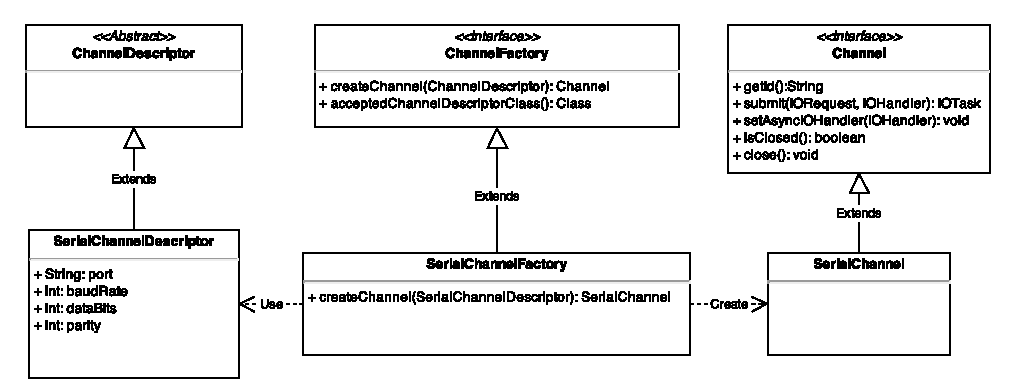
\includegraphics[width=\textwidth]{imgs/channel_factory.pdf}
\caption{Class diagram of the Channel layer}
\end{figure}

Each \texttt{ChannelFactory} is tied to a specific communication technology;
therefore, it can only accept a single class of \texttt{ChannelDescriptor}
objects. For example, the \texttt{HTTPChannelFactory} parses
\texttt{HTTPChannelDescriptor}s and creates \texttt{HTTPChannel}s, whereas an
hypothetical \texttt{SerialChannelFactory} would consume
\texttt{SerialChannelDescriptor}s to create \texttt{SerialChannel}s. Failure to
provide a suitable \texttt{ChannelDescriptor} object will cause the
\texttt{createChannel()} method to throw an
\texttt{InvalidDeviceDescriptorException}.

The \texttt{acceptedChannelDescriptorClass()} method can be used to dynamically
discover which \texttt{ChannelDescriptor} type is supported by a specific
\texttt{ChannelFactory}. This method is the fulcrum of the \texttt{Channel}
Plugin System, as it allows the Middleware to invoke the most appropriate
\texttt{ChannelFactory} using only information available at runtime.

\begin{figure}[!hbt]
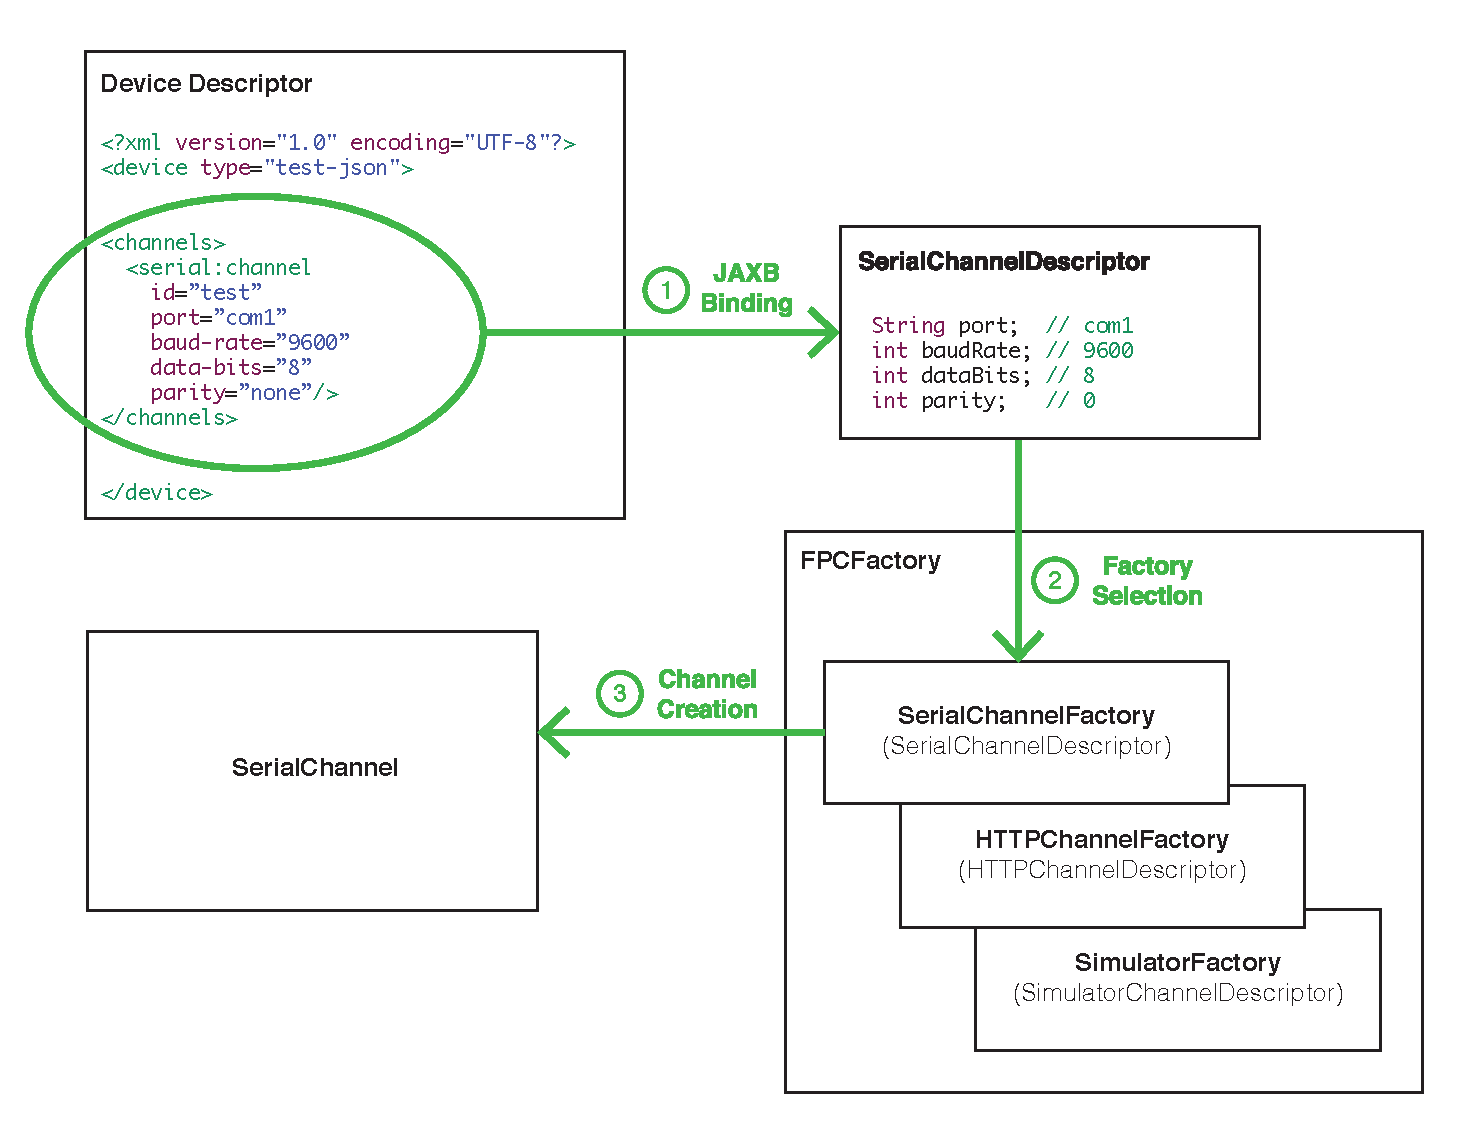
\includegraphics[width=\textwidth]{imgs/channel_creation_process.pdf}
\caption{The Channel creation process}
\label{fig:channel.creation}
{
\begin{figurenote}
This figure illustrates the \texttt{Channel} creation process executed by the
Middleware upon reception of a new Device Descriptor.  \begin{enumerate}
  \itemsep0em
  \item JAXB binds the XML Device Descriptor to an apropriate
\texttt{ChannelDescriptor} object using namespace information \item A suitable
\texttt{ChannelFactory} is selected at runtime using the
\texttt{acceptedChannelDescriptorClass()} method
  \item The information contained in the \texttt{SerialChannelDescriptor} is
used to create a new \texttt{SerialChannel} \end{enumerate}
\end{figurenote}
}
\end{figure}

\texttt{ChannelDescriptor} objects are automatically created by the
Middleware using the information contained in the Device Descriptor XML files.
This binding process is performed by the JAXB library, which is also
responsible for instantiating the correct \texttt{ChannelDescriptor} class
using XML Namespace information. Figure~\ref{fig:channel.creation} illustrates
this technique, and ties it together with the other operations described in
this section.

It is important to note that a single JVM instance running the PerLa Middleware
may host several \texttt{Channel} objects of the same type, at the same time.
Several devices can use the same communication technology, and the
\texttt{ChannelFactory} may determine that it's best to create an individual
\texttt{Channel} for each one of them. This behaviour is fostered by the new
\texttt{ChannelFactory} architecture, and is considered idiomatic design;
hence, it would not be uncommon to implement the hypothetical
\texttt{SerialChannelFactory} introduced in the previous paragraphs so that
every serial port is handled by a different \texttt{SerialChannel} instance.


\subsection{IORequest management}

\texttt{IORequest} is the base object interface employed to interact with a
sensing node connected to the Middleware. It contains two types of information:
the payload to be transferred, and \texttt{Channel}-dependent data needed for a
correct communication with the endpoint device.

\lstset{language=Java}
\begin{lstlisting}[float,floatplacement=!hbt,caption=The IORequest
interface,label={lst:iorequest}]
public interface IORequest {

	public String getId();

	public void setParameter(String name, Payload payload);
	
}
\end{lstlisting}

Every \texttt{Channel} imlementation is bundled with its own custom
\texttt{IORequest} class. Following up on previous examples, the
\texttt{HTTPChannel} package contains a \texttt{HTTPIORequest} object, whereas
the fictitious \texttt{SerialChannel} would be supplied with a
\texttt{SerialIORequest} class of request objects. This additional level of
indirection is necessary since different communication technologies require
different settings to establish end-to-end connectivity; therefore, a universal
\texttt{IORequest} object would soon prove to be a limiting factor for the
extension of the Middleware.

As shown in listing~\ref{lst:iorequest}, payload data can be set in an
\texttt{IORequest} by means of the \texttt{setParameter()} method.
\texttt{Payload}s are addressed by name, and a single \texttt{IORequest}
implementation may support several at once. The exact set of \texttt{Payload}
parameters accepted by an \texttt{IORequest} class depends on the design of its
matching \texttt{Channel}; for example, the \texttt{HTTPChannel}
implementation supports three: an `entity' payload (request body), a `query'
payload (an URL-encoded string), and a `path' payload (a path component used to
identify a single resource accessible from the base URL).

\texttt{IORequest}s are disposable objects; they are created, submitted to a
\texttt{Channel}, and garbage collected once the communication is over.
Creation is performed by means of a factory interface dubbed
\texttt{IORequestBuilder}, which allows the Middleware to build new copies of
an \texttt{IORequest} from a fixed template. It is important to note that
request objects built using this technique do not contain \texttt{Payload}
parameters; these are to be added manually before subbmitting the
\texttt{IORequest} to a \texttt{Channel}.

Besides \texttt{IORequest} creation, the \texttt{IORequestBuilder} interface
can be used to dynamically discover which \texttt{Payload} parameters are
supported by an \texttt{IORequest}. This functionality, exposed through the
\texttt{getParameterList()} method, is a crucial component of the Middleware
Plugin System, as it allows \textit{Script} instructions to determine whether
an \texttt{IORequest} was populated with all the necessary \texttt{Payload}
parameters or not. This concept will be the subject of further analysis in
section~\ref{sec:components.script}.

A single device connected to the PerLa Middleware is generally managed using
several \texttt{IORequestBuilder}s, any one of which is responsible for
creating a request object suitable to control a single aspect of
the interaction with the endpoint. The main advantage brought by this
templating mechanism is that \texttt{Channel}-related configuration settings
are only specified once, hence the same \texttt{IORequest} structure can be
reused multiple times to transport different payload information.

\lstset{language=Java}
\begin{lstlisting}[float,floatplacement=!hbt,caption=The IORequestBuilder
interface,label={lst:iorequestbuilder}]
public interface IORequestBuilder {

	public String getRequestId();

	public IORequest create();

	public abstract List<IORequestParameter> getParameterList();

	public static class IORequestParameter {

		public String getName() {
			return name;
		}

		public boolean isMandatory() {
			return mandatory;
		}

	}
}
\end{lstlisting}

REST APIs are an excellent use case to demonstrate the aforementioned concept,
as every operation on a RESTful resource can be easily abstracted using an
appropriately configured request builder. By using
\texttt{HTTPIORequestBuilder} objects, HTTP protocol information (base URL,
method, header, \ldots) are specified one single time only for
every REST endpoint. Once this step is done, the API can be invoked just by
building new \texttt{IORequest}s and submitting them to a \texttt{HTTPChannel}.

\begin{figure}[!hbt]
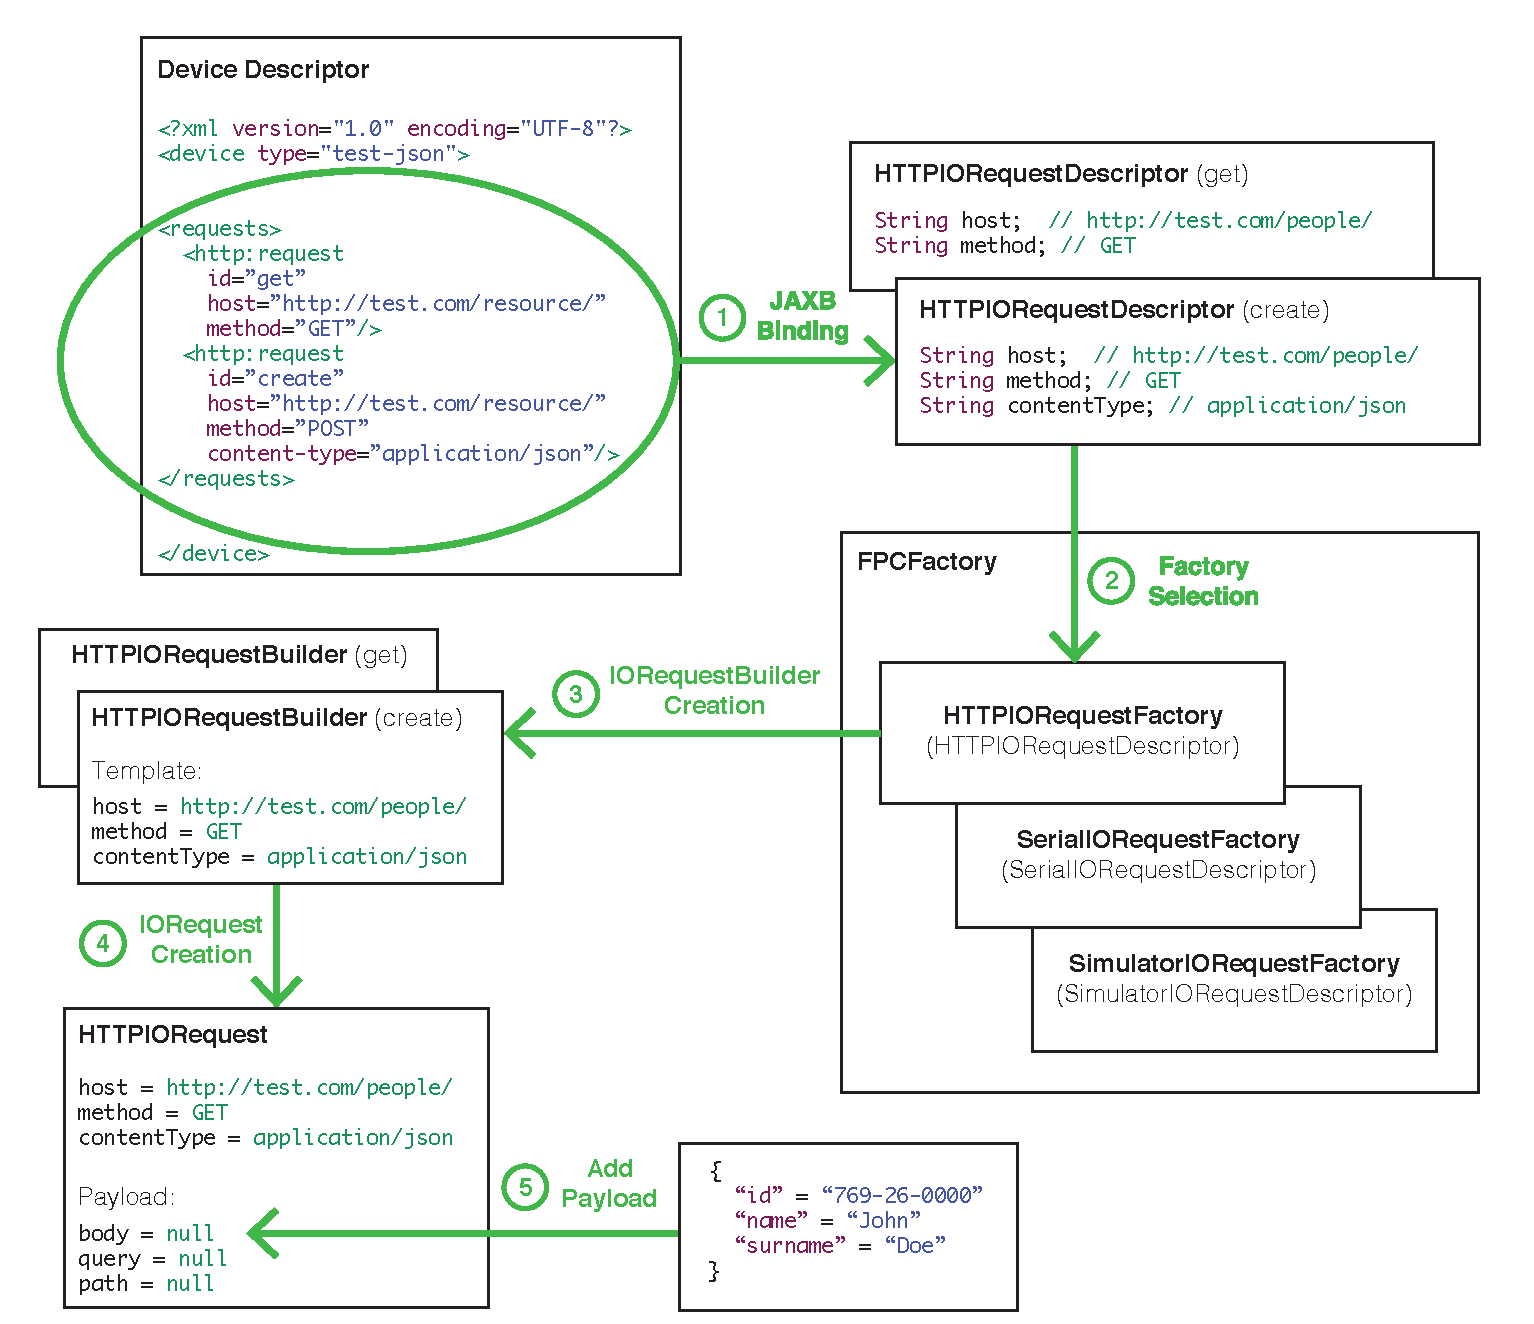
\includegraphics[width=\textwidth]{imgs/iorequest_creation_process.pdf}
\caption{The IORequest creation process}
\label{fig:iorequest.creation}
{
\begin{figurenote}
This figure illustrates the autonomous creation of \texttt{IORequest} objects.
Steps 1 to 3 are performed only once after receiving the Device Descriptor,
whereas steps 4 and 5 are repeated every time the REST API is to be invoked.
\begin{enumerate}
  \itemsep0em
  \item JAXB binds the XML Device Descriptor to an apropriate
\texttt{IORequestDescriptor} object using namespace information \item A
suitable \texttt{IORequestBuilderFactory} is selected at runtime using the
\texttt{acceptedIORequestDescriptorClass()} method
  \item The information contained in the \texttt{IORequestDescriptor} is used
to create a new \texttt{IORequestBuilder} \item The \texttt{IORequestBuilder}
is used to create new \texttt{IORequest} copies using the internal template
  \item The newly created \texttt{IORequest} objects can be populated with
\texttt{Payload} parameters as needed \end{enumerate}
\end{figurenote}
}
\end{figure}

\texttt{IORequestBuilder}s are created by means of an
\texttt{IORequestBuilderFactory}, an object that implements the now familiar
Factory design pattern. Creation proceeds as follows: the request template is
loaded from an XML Device Descriptor, bound to an appropriate
\texttt{IORequestDescriptor}, and processed by the
\texttt{IORequestBuilderFactory} to create the corresponding
\texttt{IORequestBuilder}. Similarly to what already seen in the previous
section, every \texttt{IORequestBuilderFactory} implements an
\texttt{acceptedIORequestDescriptorClass()} method, which can be used to
dynamically determine if a factory object can parse a specific type of
\texttt{IORequestDescriptor}. It should come as no surprise that every
\texttt{IORequestBuilder} class is provided with complementary
\texttt{IORequestBuilderFactory} and \texttt{IORequestDescriptor}
implementations.

\begin{figure}[!hbt]
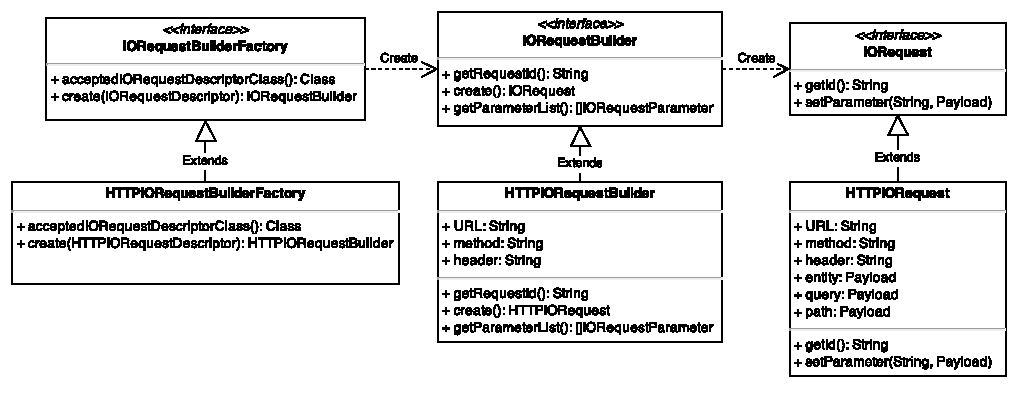
\includegraphics[width=\textwidth]{imgs/iorequest.pdf}
\caption{The extended IORequest class diagram. For additional information about
the IORequestParameter object consult listing 1.5.} \label{fig:iorequest.class}
\end{figure}


\subsection{Handling asynchronous I/O operations}

As mentioned in previous sections, communication with a device connected to the
PerLa Middleware is achieved by means of the \texttt{Channel.submit()} method.
Invocations of \texttt{submit()} are non-blocking; control flow is immediately
returned to the caller, thus allowing other computations to be performed while
the requested I/O operation is being processed.

As can be seen in listing~\ref{lst:channel}, \texttt{submit()} requires two
parameters: an \texttt{IORequest} and an \texttt{IOHandler} callback object.
The former specifies which I/O operation is to be performed, while the latter
allows the caller to be asynchronously notified of its completion.

The \texttt{IOHandler} interface is composed of two methods, namely
\texttt{complete()} and \texttt{error()}, which are invoked when processing of
an I/O operation comes to an end. It is important to note that both these
methods always carry context information in the form of an \texttt{IORequest},
which is guaranteed to be the same exact object used for starting the I/O
operation whose completion is being notified. For this reason,
\texttt{IOHandler} can be considered the nexus of the asynchronous invocation
model, as it connects \texttt{IORequest} objects with the outcome of the
corresponding I/O operation performed by the \texttt{Channel}.

\lstset{language=Java}
\begin{lstlisting}[float,floatplacement=H,caption=The IOHandler
interface,label={lst:iohandler}]
public interface IOHandler {
	public void complete(IORequest request, Optional<Payload> result);
	
	public void error(IORequest request, Throwable cause);
}
\end{lstlisting}

\lstset{language=Java}
\begin{lstlisting}[float,floatplacement=!hbt,caption=The IOTask
interface,label={lst:iotask}]
public interface IOTask {
	public void cancel();
	
	public IORequest getRequest();
	
	public boolean isCancelled();
	
	public boolean isDone();
}
\end{lstlisting}

Semantically, an invocation of the \texttt{complete()} method is always
associated with the successful termination of an I/O operation. As shown in
listing~\ref{lst:iohandler}, this method includes an optional \texttt{Payload}
object, that contains all data received from the endpoint device. A call to
\texttt{complete()} with an empty \texttt{Payload} indicates that the I/O
operation was completed without errors, but no data was received. Conversely,
an invocation of the \texttt{error()} method indicates that the I/O operation
was aborted before completion. In this case the cause of failure is always
notified through the \texttt{cause} parameter.

From the point of view the Java memory model, the \texttt{Channel.submit()}
creates a happens-before relationship with \texttt{IOHandler.complete()} and
\texttt{IOHandler.error()}, viz. any side effect generated by the code that led
to the \texttt{submit()} invocation is guaranteed to be visible in the
\texttt{complete()} and \texttt{error()} callback methods.

Asynchrous execution does not imply loss of control; ongoing I/O operations can
be monitored or cancelled by means of the \texttt{IOTask} object acquired upon
submitting an \texttt{IORequest}. Listing~\ref{lst:iotask} shows all methods of
the \texttt{IOTask} interface; method names are self explanatory, and the
reader should be able to deduce their purpose just by analyzing their 
signature. The only nuance worth mentioning is that
\texttt{isCancelled()} always implies \texttt{isDone()} (i.e., all cancelled
I/O operations are also complete), while the opposite does not hold (i.e., not
all complete I/O operations were cancelled).

\begin{figure}[!hbt]
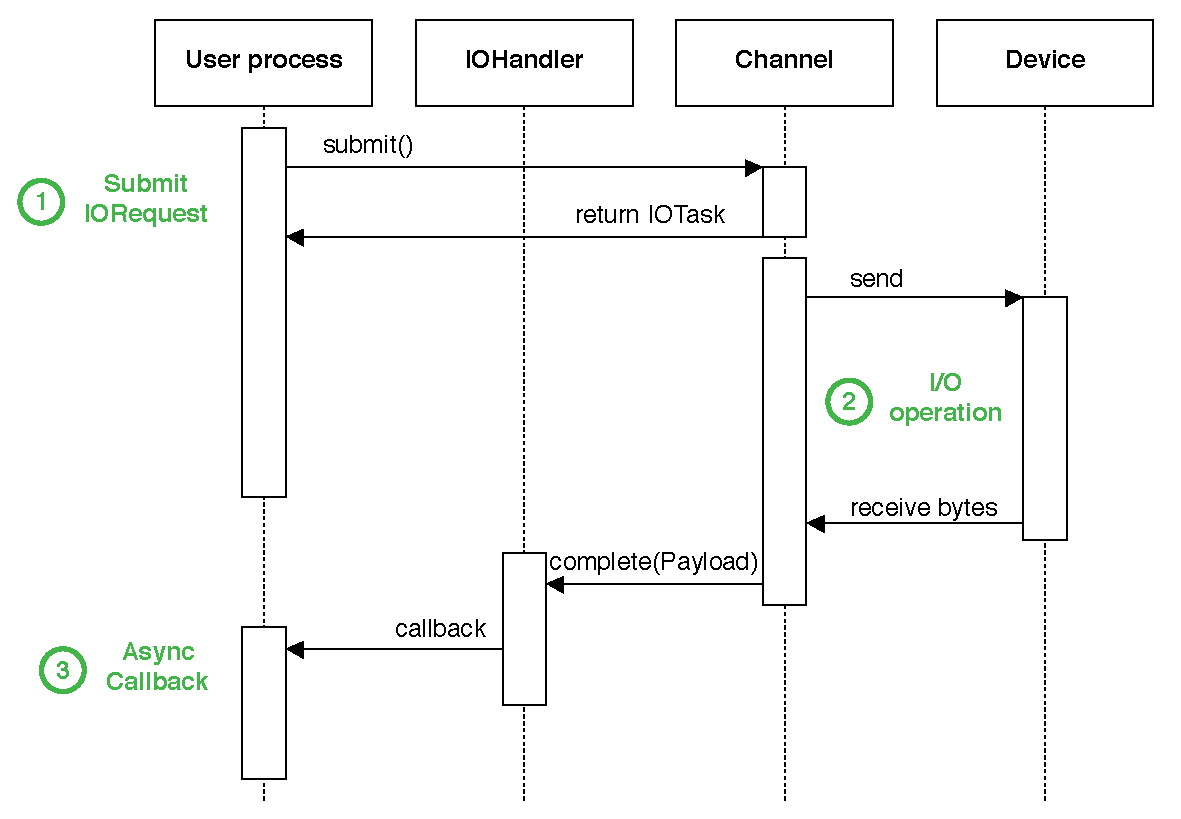
\includegraphics[width=\textwidth]{imgs/async_channel_sequence.pdf}
\caption{Sequence diagram of an asynchronous I/O operation. Note that the user
process and the I/O operation are executed in parallel.}
\label{fig:channel.async}
\end{figure}

The \texttt{Channel} interface is also designed to manage completely
asynchronous I/O operations, namely communication efforts spontaneously
initiated by the remote device. This communication model is popular among WSNs,
as it is often employed to handle periodic data streams or events happening
at irregular intervals. Such I/O operations can be handled through a catch-all
\texttt{IOHandler} set with the \texttt{setAsyncIOHandler()} method
(listing~\ref{lst:channel}). Since the communication is not initiated by the
Middleware, the \texttt{complete()} and \texttt{error()} callback methods will
be invoked with the \texttt{IORequest} parameter set to \texttt{null}.


\section{Handling data}
\label{sec:components.mapper}

\texttt{Payload} is a container for raw sequences of bytes. In spite of its
semplicity, this class forms the foundation of the entire PerLa Middleware, as
it is the vessel that conveys all information passing through the
\texttt{Channel} interface.

The data encapsulated in a \texttt{Payload} object is accessed one byte at a
time; this granularity level is ideal for the implemention of an I/O access
layer, whose sole concern consists in the transmission of information between
two endpoints, but is not suited to other forms of data management. Processing
the information contained in a \texttt{Payload} can be unwieldy and
unnecessarily complex; the byte-oriented interface doesn't provide any facility
for leveraging the underlying structure of the enclosed data, and even a simple
action like retrieving a value in a complex data structure can easily become a
daunting task.


\subsection{The Message interface}

\texttt{Message}s are structured data containers that enclose a group of
individual items called fields. The chief advantage that this data structure
provides over the simpler \texttt{Payload} object consists in the possibility
of addressing information by field name, a convenient feature that dispenses
with the burden of managing data in byte-sized chunks. The methods available in
the \texttt{Message} interface are shown in listing~\ref{lst:message}.

\lstset{language=Java}
\begin{lstlisting}[float,floatplacement=!hbt,caption=The Message
interface,label={lst:message}]
public interface Message {

    public String getType();

    public boolean hasField(String name);

    public Object getField(String name)
                throws IllegalArgumentException;

    public void setField(String name, Object value)
                throws IllegalArgumentException;

    public void appendElement(String name,Object element)
                throws IllegalArgumentException;

    public boolean validate();

}
\end{lstlisting}

The specific structure of a \texttt{Message} is defined by its type, which can
be queried through the \texttt{getType()} method. This property unequivocally
identifies the set of fields contained in a \texttt{Message} in terms of field
\textbf{name}, field \textbf{type} and field \textbf{qualifier}.

The field \textbf{name} is a textual attribute that uniquely identifies one
specific data item in the scope of a single \texttt{Message}. It can be used to
retrieve or set the value of a field through the \texttt{getField()} and
\texttt{setField()} methods respectively.

The \textbf{type} attribute defines the set of legal values that can be stored
in a field, together with the operations that are allowed on those values. It
is worth mentioning that this information is used to statically verify the type
safety of nearly all data management operations performed on a \texttt{Message}
(consult section~\ref{sec:components.script} for additional information). The
PerLa Middleware currently supports six primitive types:

\begin{itemize}

  \item \textbf{INTEGER}: a 32 bit signed two's complement integral data type

  \item \textbf{FLOAT}: a single-precision 32 bit IEEE 745 floating point

  \item \textbf{BOOLEAN}: a type with only two values, true or false

  \item \textbf{STRING}: a string of characters with UTF-16 encoding

  \item \textbf{TIMESTAMP}: a date with timezone, currently implemented using
      Java's \texttt{ZonedDateTime} class.

  \item \textbf{ID}: a unique label that identifies a single node connected in
      a PerLa managed network. The current implementation uses a 32 bit
      integer. 

\end{itemize}

Besides the data types presented above, fields can also be configured to hold
nested \texttt{Message}s. In this case, the type attribute must be set to the
particular type of \texttt{Message} that is to be stored in the field. 

The \textbf{qualifier} attribute is employed to define additional field
properties. It can be set to one of the following values:

\begin{itemize}

  \item \textbf{SIMPLE}: a normal field whose value can be altered and
      retrieved using the \texttt{setField()} and \texttt{getField()} methods
      respectively.

  \item \textbf{LIST}: a field that can hold multiple elements of the same
      type. New values can be added with the \texttt{appendElement()} method,
      and the entire list can be retrieved through the conventional
      \texttt{getField()} method. List-qualified fields preserve the order of
      insertion of the individual elements.

  \item \textbf{STATIC}: a field whose value is statically set when the
      \texttt{Message} type is declared. Any attempt to modify a
      statically-qualified field with either the \texttt{setField()} or the
      \texttt{appendElement()} methods will cause an exception to be thrown. It
      is important to note that static field values are set on a per-type
      basis; this means that all \texttt{Message}s of the same type will share
      the same field values for each static field (if any).
      
\end{itemize}


\subsection{Working with Messages: the Mapper interface}

\texttt{Message} objects are managed by the \texttt{Mapper} component. Its
interface, available in listing~\ref{lst:mapper}, groups all the
functionalities needed to handle a specific variety of structured information.
The one-to-one relationship between \texttt{Mapper}s and data types is
epitomized by the \texttt{getMessageType()} method, whose return value
indicates which \texttt{Message} class is supported by a particular
\texttt{Mapper}. This method is extensively employed by the Middleware to sift
through a collection of \texttt{Mapper}s, in order to find one that is best
suited for handling the information currently being processed.

\lstset{language=Java}
\begin{lstlisting}[float,floatplacement=!hbt,caption=The Mapper
interface,label={lst:mapper}]
public interface Mapper {

    public String getMessageType();

    public FieldDescriptor getFieldDescriptor(String name);

    public Collection<FieldDescriptor> getFieldDescriptors();

    public FpcMessage createMessage();

    public FpcMessage unmarshal(Payload payload);

    public Payload marshal(FpcMessage message);

}
\end{lstlisting}

Interactions with a \texttt{Mapper} usually begin with a call to the
\texttt{createMessage()} method, whose execution results in the creation of an
empty \texttt{Message} instance. Despite its unsuprising outcome, this method
draws once again our attention to the close relationship between
\texttt{Mapper}s and data types. Every \texttt{Mapper} instance is in fact
committed to the management of a precise class of information, hence all
\texttt{Message}s created with the \texttt{createMessage()} method will share
the same data type property, and, consequently, the same set of fields. The
interdependence between a \texttt{Mapper} and its assigned type is accentuated
even further by the \texttt{getFieldDescriptor()} and
\texttt{getFieldDescriptors()} methods, which can be used to analyze the
internal field structure characterizing all \texttt{Message} objects that the
\texttt{Mapper} creates. This introspective capability is extensively exploited
in the Execution Engine to check whether a \textit{Script} is type-safe or not
(see section~\ref{sec:components.script} for further details).

As explained in the introductory paragraphs of this section, \texttt{Message}
objects are a convenience introduced for simplifying data management operations
in the PerLa Middleware. They provide structured access to information, a
familiar set of primitive data types, and a selection of tools for combining
basic values into complex data structures. In spite of these advantages, the
\texttt{Message} interface is a high level abstraction that cannot be employed
where a \texttt{Payload} is expected, since its contents are not directly
accessible as a simple sequence of bytes; as a consequence, \texttt{Message}s
can't be used for any kind of I/O operation. This structural gap is bridged by
the \texttt{marshal()} and \texttt{unmarshal()} methods of the \texttt{Mapper}
interface. As can be seen by analyzing their respective signatures, these two
methods can be used to convert \texttt{Message} objects into \texttt{Payload}s
and vice-versa. This additional \texttt{Mapper} functionality brings to light
yet another aspect of the PerLa data management layer, namely its ability to
work with different representations of binary data.

Every \texttt{Mapper} is in fact created to support a single data format;
\texttt{JSONMapper} instances, for example, handle JSON-formatted byte streams,
whereas \texttt{URLEncodedMapper}s specialize in the conversion of URL-encoded
HTTP entities. The structure of the \texttt{Message}s created by a
\texttt{Mapper} and the data format they can be marshalled unto are not
orthogonal concerns, as the choice of a specific binary representation may
prevent the use of some of the previously discussed field attributes. The
URL-encoded format, for example, is defined as a flat collection of key-value
pairs, with no support for nested data structures; hence, the corresponding
\texttt{URLEncodedMapper} class could never be used to create and manage
\texttt{Message}s with nested fields. The close connection between a
\texttt{Message} and its corresponding binary format manifests itself in the
design of the \texttt{Mapper} component, specifically in the decision to
coalesce the marshalling/unmarshalling mechanism, and the more general
\texttt{Message} management methods (\texttt{createMessage()},
\texttt{getFieldDescriptors()}), under the same interface. The specific
methodology for creating \texttt{Mapper} objects, and for defining their
distinctive data format and \texttt{Message} type, will be subject of
additional discussion in the remainder of this chapter.

\begin{figure}[h!]
    \centering
    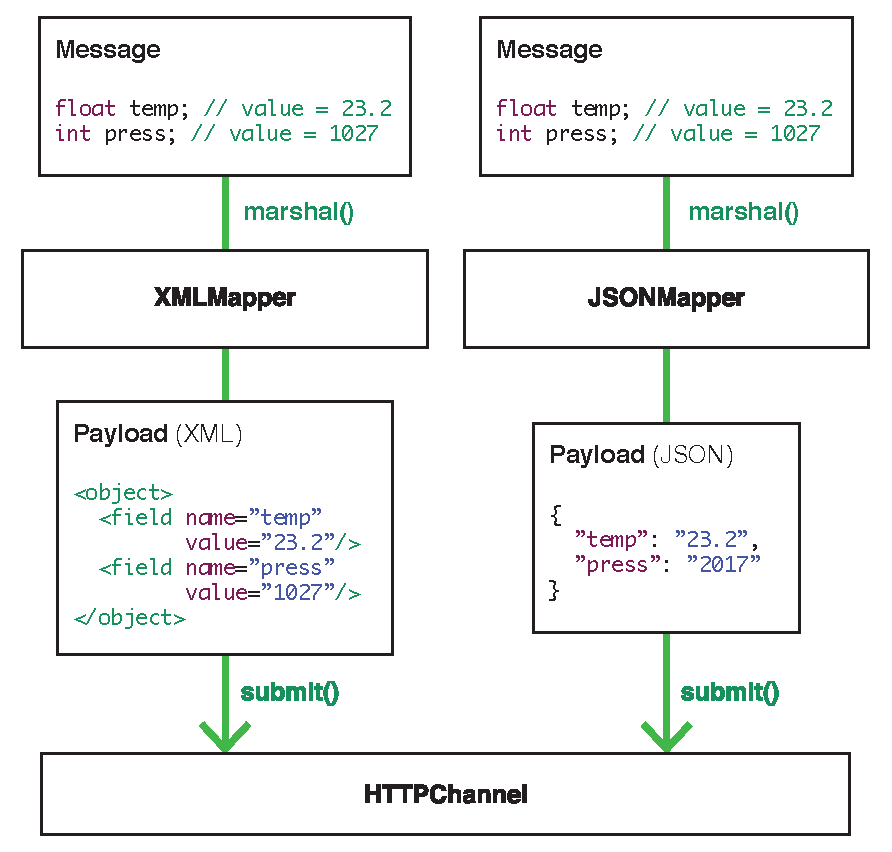
\includegraphics[scale=0.8]{imgs/mapper_channel.pdf}
    \caption{Using a single \texttt{Channel} to transmit data marshalled with
    different \texttt{Mapper}s}
    \label{fig:mapper_channel}
\end{figure}

Before this section comes to an end, it is worth putting into context the role
occupied by the \texttt{Mapper} inside the PerLa Middleware. The additional
decoupling provided by the \texttt{Mapper} builds over the pluggable
\texttt{Channel} interface, thus allowing the payload format to be selected
independently of the I/O stack.  This is an important characteristic of the
Middleware design, as even the simplest communication protocol usually requires
several \texttt{Message} structures, viz. several \texttt{Mapper}s, for
exchanging data between two endpoints.


\subsection{Creating Mappers and defining Message structures}

New \texttt{Mapper} objects are created by means of the \texttt{MapperFactory}
interface.

\lstset{language=Java}
\begin{lstlisting}[float,floatplacement=!hbt,caption=The Mapper Factory
interface,label={lst:mapperFactory}]
public interface MapperFactory {

    public Class<? extends MessageDescriptor>
        acceptedMessageDescriptorClass();

    public Mapper createMapper(MessageDescriptor descriptor,
        Map<String, Mapper> mapperMap, ClassPool classPool)
                    throws InvalidDeviceDescriptorException;

}
\end{lstlisting}

Its design follows the same concepts explained in previous sections; the
\texttt{acceptedMessageDescriptorClass()} method returns the type of
\texttt{MessageDescriptor} objects that can be used with the
\texttt{MapperFactory}, while the \texttt{createMapper()} method consumes a
\texttt{MessageDescriptor} to create a \texttt{Mapper}. However, differently
from all factory components described so far, the creation of a new object
calls for two additional parameters other than the descriptor itself: a
\texttt{ClassPool}, and a map of \texttt{Mapper}s. These extra items contain a
reference to previously built \texttt{Mapper}s, and can be used to check
whether nested \texttt{Message} fields are properly declared or not.

The \texttt{MapperFactory} interface is an additional extension point available
to PerLa users, and can be leveraged to introduce support for new binary
formats and information encoding schemes. As a consequence, every installation
of the Middleware will contain a wide variety of \texttt{MapperFactory}
implementations, each of which is dedicated to a single data format. Instances
of the previously introduced JSON and URL-Encoded mappers, for example, are
created by two distinct \texttt{MapperFactory} objects, namely
\texttt{JSONMapperFactory} and \texttt{URLEncodedMapperFactory}. This design is
a substantial improvement on the previous middleware architecture, as it
ensures that every \texttt{MapperFactory} object is responsible for managing
the quirks of only a single data format.

Moreover, every \texttt{MapperFactory} implementation is bundled with a custom
\texttt{MessageDescriptor} object, whose class name is exposed by the
aforementioned \texttt{acceptedMessageDescriptorClass()} method. The additional
complexity deriving from this design choice is more than made up for in type
safety and flexibility, as each different \texttt{MessageDescriptor} may be
implemented to closely represent the idiosyncratic characteristics of its
corresponding data format. A concrete example of this concept comes from the
\texttt{URLEncodedMessageDescriptor} class, which prevents the creation of
\texttt{Message}s that don't comply with the URL-encoded format by disallowing
non-primitive fields. Having multiple \texttt{MessageDescriptor}s also means
that different \texttt{Message}s are not forced to abide by the same set of
rules; the limits imposed on URL-encoded messages are not universal, and in
fact the \texttt{JSONMessageDescriptor} refrains from applying them.
Furthermore, \texttt{MessageDescriptor} objects can adopt a custom lexicon for
expressing the PerLa-specific concepts of \textit{message}, \textit{field} and
\textit{field type}. Take for example listings \ref{lst:jsonmessage} and
\ref{lst:urlencodedmessage}. These two XML snippets show how the vocabulary
employed in message declarations varies with the data format (field are dubbed
\textit{member} in JSON, and \textit{parameter} in URL-Encoded strings). Using
a terminology that best suits the actual data format makes \texttt{Message}
declarations idiomatic, reminiscent of the corresponding real-world objects and
therefore easier to use.

\lstset{language=XML}
\begin{lstlisting}[float,floatplacement=!hbt,caption={A compound JSON message
        declared using the JSONMessageDescriptor (XML notation). Note that the
        data type of all fields inside \texttt{weather} message is a reference
        to a previously declared \texttt{Message}.
},label={lst:jsonmessage}]

<js:object id="coord">
    <js:member name="lon" type="string"/>
    <js:member name="lat" type="string"/>
</js:object>

<js:object id="main">
        <js:member name="temp" type="float"/>
        <js:member name="pressure" type="float"/>
        <js:member name="humidity" type="float"/>
        <js:member name="temp_min" type="float"/>
        <js:member name="temp_max" type="float"/>
</js:object>

<js:object id="wind">
        <js:member name="speed" type="float"/>
        <js:member name="deg" type="float"/>
</js:object>

<js:object id="weather">
        <js:member name="coord" type="coord"/>
        <js:member name="main" type="main"/>
        <js:member name="wind" type="wind"/>
</js:object>

\end{lstlisting}


\lstset{language=XML}
\begin{lstlisting}[float,floatplacement=!hbt,caption={An URLEncoded message
declaration. Thanks to the custom \texttt{URLEncodedMessageDescriptor}, trying
to create a non-primitive field results in an exception. Note the custom
\texttt{format} attribute on the timestamp field, which is employed to define
the encoding format for dates and times},label={lst:urlencodedmessage}]

<ue:message id="urlencoded_message">
        <ue:parameter name="temperature" type="float"/>
        <ue:parameter name="pressure" type="float"/>
        <ue:parameter name="location" type="string"/>
        <ue:parameter name="key" qualifier="static" type="integer" value="5"/>
        <ue:parameter name="timestamp" type="timestamp" format="d MMM uuuu HH:mm"/>
</ue:message>

\end{lstlisting}


\subsection{Managing multiple message types}

It is not uncommon for a single device to communicate using multiple message
formats; developers may choose to encapsulate different information inside
different data structures, which the receiver must correctly identify to
decipher their contents. In such cases, every \texttt{Message} exchanged
between the two endpoints is tagged with a data type value, i.e., a common
field that advertises the type of information being transferred. This technique
is widespread among firmware developers, since it can be easily implemented
with most programming languages (C/C++ support it by design through
\texttt{tagged unions}).

The PerLa Middleware implements various techniques to cope with sensor nodes
that communicate using multiple message formats. First of all, only the data
structures that can actually be received are considered when unmarshalling a
byte stream; if under the current conditions a device only sends a subset of
its available message types, then the Middleware can immediately rule out the
unmatching ones. As it will be discussed later, a collection of expected data
formats is automatically curated by the \texttt{FPC} by cross-comparing
information excerpted from the Device Descriptor with the current device
status. It should be clear that this technique alone is not enough to cover all
practical use cases, as it falls short as soon as a device starts sending two
or more message varieties concurrenty; in such scenarios, PerLa needs to search
for clues that will help it recognize how the bytes being received are
structured. These clues take the form of \textit{static} fields. When faced
with an ambiguous situation, the \texttt{FPC} will try unmarshal the bytes
received into all expected data types. A congruency check will then be
performed on the resulting \texttt{Message}s: the data can be considered
correctly decoded only when all its static fields match the corresponding
Device Descriptor declaration. This methodology can be employed to interact
with sensor nodes that make use of tagged data structures. 


\section{Data management: Scripts}
\label{sec:components.script}

\texttt{Channel}s, \texttt{Payload}s, \texttt{Mapper}s and \texttt{Message}s
are the core components used by PerLa to exchange data with nodes of a
Pervasive System. They provide the supporting infrastructure through which
information can be serialized, transmitted and faithfully reconstructed at the
receiving endpoint. Taken together, these components implement an adaptable
transport layer, whose features can be tailored around each device connected to
the Middleware: combine a \texttt{HTTPChannel} with a \texttt{JSONMapper} to
obtain a network stack for RESTful services; swap the data layer with an
\texttt{XMLMapper} if the format changes; add a \texttt{ZigbeeChannel} and a
\texttt{StructMapper} to communicate with low-powered devices in a mesh
network. In spite of their individual capabilities, all these components are
not enough to glean information from a Sensor Network. The interaction with a
sensor node requires far more than a transport layer; in fact it can only occur
when data transfer operations follow a strict set of rules, i.e., an
\textit{application protocol}. \texttt{Channel}s, \texttt{Mapper}s and
\texttt{Message}s provide no more than the basic building blocks needed for the
interaction, but their use is to be tightly orchestrated before any purposeful
exchange of information can take place.

PerLa \textit{Script}s, just referred as \textit{Script}s in the remainder of
this document, implement the kind of structural scaffolding required to
organize a series of primitive data management operations into a
self-contained, reusable procedure. Their purpose in the PerLa Middleware is
twofold: first, to issue commands that conform to the specific protocols used
in a Pervasive Systems; second, to act as an impedance matcher between the
structured information collected from a sensor network and the record-oriented
output of an \texttt{FPC}. The PerLa scripting language is one of the most
distinctive features of the new Middleware design; a procedural programming
tool that can be used to complement and enrich the declarative nature of the
Device Descriptor. \textit{Script}s improve the reusability of all existing and
future Middleware components, as they can be used to adjust the output of a
computation before it's used as the input of another one.

\begin{figure}[h!]
    \centering
    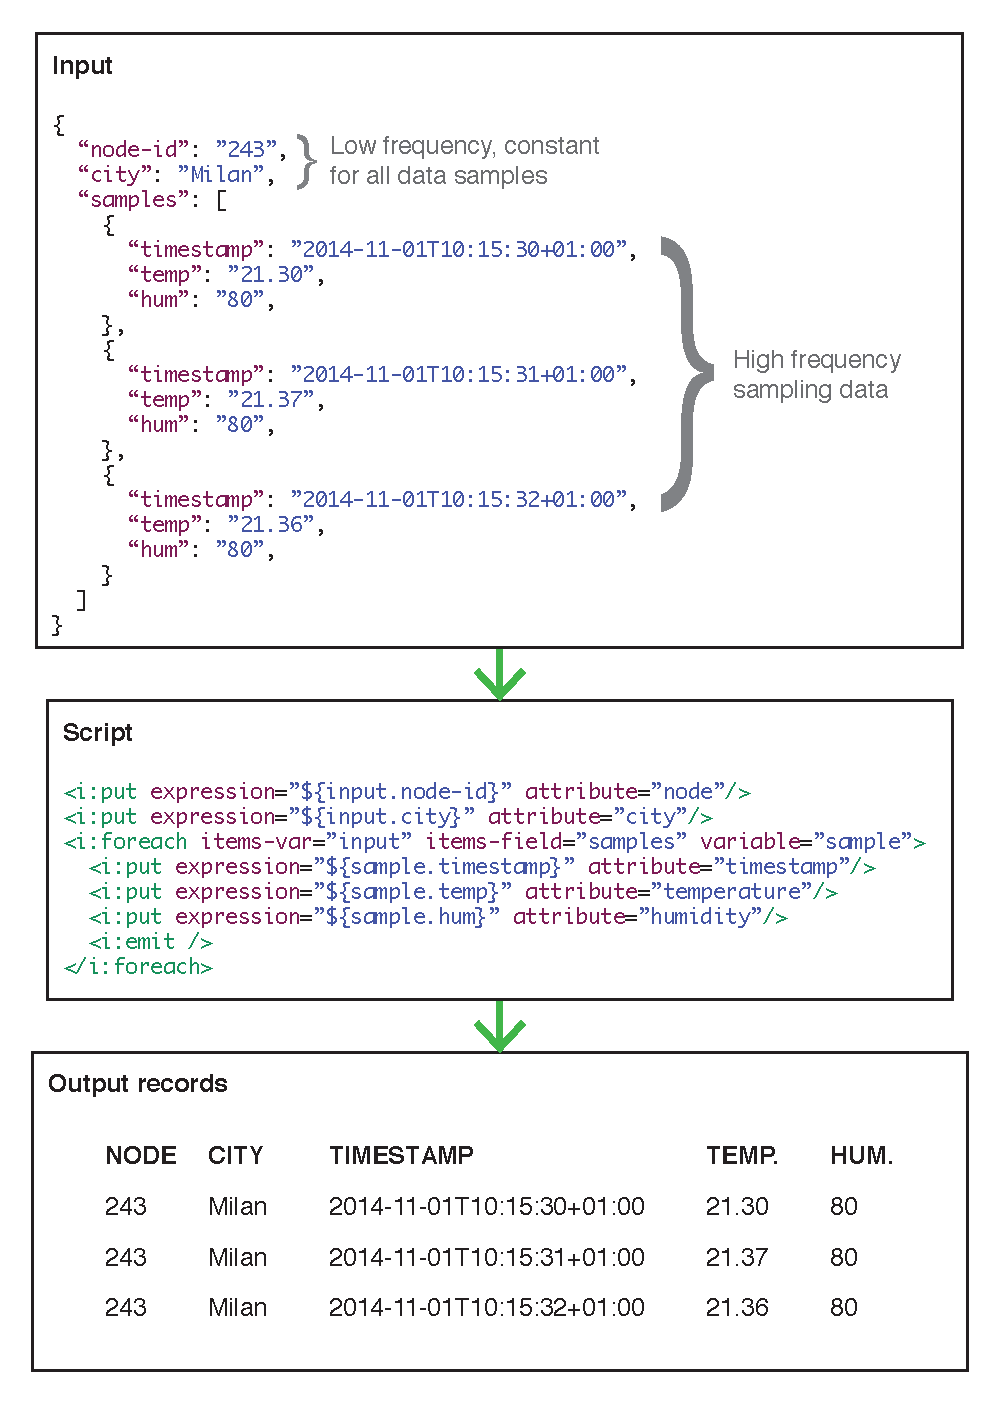
\includegraphics[scale=0.8]{imgs/script_unrolling.pdf}
    \caption{Flattening the content of a nested JSON data structure with a
    PerLa \texttt{Script}}
    \label{fig:script_unrolling}
\end{figure}

An archetypal example of this concept is given in
figure~\ref{fig:script_unrolling}. This \textit{Script} solves a recurring
impedance matching problem: a device that stores multiple samples into a common
data structure, and sends them with a single transmission in order to conserve
battery power. The result of such aggregation can't be coerced into a sequence
of records as-is, as more often than not it contains a mixture of both high
frequency and low frequency information (and indeed it does in the current
example). The PerLa scripting language can be used to unroll the high frequency
content, complement it with the information that remains constant for all
samples, and output the resulting records one by one; all without having to
resort to a bespoken \texttt{Mapper} implementation, as it would prove
necessary if the former Middleware were used instead. Moreover, this same
script can be easily employed to handle similar aggregation patterns with
little or none modifications, as it doesn't depend on any particular
\texttt{Channel}, \texttt{Mapper} or \texttt{Message} implementation.

PerLa \textit{Scripts} are also used to address minor compatibility problems
that may arise when authoring new Device Descriptors; they can wrap an existing
Middleware component and adapt its behaviour to handle an unforseen usage
scenario, convert information between different units of measure, alter a
\texttt{Message} before it is sent to the intended recipient, or compute
aggregations. It is important to note that \textit{Scripts} are slower than
pure Java code; an excessive usage in data intensive, real-time applications
should be carefully avoided, as it may negatively affect the performance of the
entire Middleware. End users are therefore invited to thoroughly test and
benchmark their Device Descriptors to eliminate any potential bottleneck before
deployment.


\subsection{Anatomy of a PerLa Script}

PerLa \texttt{Script} is a full-fledged imperative programming language
composed of data management instructions, control flow statements and a
powerful expression language. Procedures written in PerLa \texttt{Script} are
processed by the \texttt{Script Engine}, a Middleware module that reads,
interprets and executes script instructions. Instructions are specified using a
proprietary XML syntax, specifically designed to allow PerLa \texttt{Scripts}
to be directly embedded in a Device Descriptor. Conflicts with potentially
similar XML tags and attributes are avoided through the
\texttt{http://perla.dei.org/device/instructions} namespace, which is commonly
associated with the ``\texttt{<i:}'' prefix. PerLa developers are invited to
follow this convention, as the use of a different namespace prefix may create
confusion among end users and future Device Descriptor maintainers. 

Every \texttt{Script} instruction is composed of a \textit{name}, a textual
property that identifies a specific type of computation, and a list of
\textit{parameters}, name-value pairs that customize its runtime behaviour.
With the exception of the \texttt{submit} instruction, whose unconventional
characteristics are described in the remainder of this section, parameters are
always defined using the standard XML attribute syntax.  PerLa \texttt{Scripts}
currently support two different types of parameter values: \textit{literals}
and \textit{expressions}. Literals are simple textual strings, which are used
as-is by the execution engine to express constant concepts like variable names
or immutable values. Expressions, on the other hand, are combinations of
variables, operators, functions and constants, whose evaluation produces a new
result value. Differently from literals, expressions are prefixed by the \$
sign and enclosed in curly braces (\lstinline!${ ... }!); this cue is employed
by the execution engine to determine whether an instruction parameter has to be
pre-processed or not prior to being used.  Expressions can be used to perform
the following actions:

\begin{itemize}
        
    \item Arithmetic operations (sum, subtration, product, division, modulo)

    \item Logical operations (or, and, not)

    \item Comparisons (\lstinline$<, >, !=, <=, >=$)

    \item Access \texttt{Message} fields (dot operator). Multiple dot operators
        may be applied in succession to access a specific value buried inside a
        complex data structure (e.g., the expression
        \lstinline!${result.environment.temperature}! is used to traverse 3
        nesting levels).

    \item Retrieve \texttt{Script} arguments through the built-in \texttt{args}
        associative array. This feature can be leveraged to create parametric
        \texttt{Script}s that dynamically adapt to the user's requests.

\end{itemize}

Whether a certain parameter can be specified as a literal, as an expression, or
both, depends entirely on the instruction in which it is employed. This
information, along with other useful details regarding the PerLa Scripting
language, is available in the following instruction compendium.

\subsubsection{\texttt{var} instruction}

\textbf{Description}

Declares a new variable. This instruction requires two mandatory parameters:

\begin{itemize}

    \item \textbf{name:} The variable name, namely a textual identifier used to
        reference the variable in later instructions. It must be unique in the
        scope of a single script.

    \item \textbf{type:} The type of data that can be stored inside the newly
        created variable. It can be set to one of the six PerLa primitive data
        types, or to a user-defined  message type.

\end{itemize}

\textbf{Usage examples}

Creates a new variable named \texttt{count} of primitive type \texttt{integer}.

\lstset{language=XML}
\begin{lstlisting}
<i:var name="count" type="integer"/>
\end{lstlisting}

Creates a new variable named \texttt{cmd} of complex type
\texttt{node\_command}, whose declaration is omitted for brevity reasons.

\lstset{language=XML}
\begin{lstlisting}
<i:var name="cmd" type="node_command"/>
\end{lstlisting}

\subsection{\texttt{set} instruction}

\textbf{Description}

Sets the contents of a variable to a new value. The optional \texttt{field}
parameter can be used whenever the user needs to modify a specific field in a
variable of complex type.

\begin{itemize}

    \item \textbf{variable:} Name of the variable to be modified.

    \item \textbf{field (optional):} An optional parameter that can be used to
        select the specific field to set in a variable of complex type.

    \item \textbf{value:} The new value of the variable. This parameter may
        be either a literal value or an expression.

\end{itemize}

\textbf{Usage examples}

Sets the previously defined \texttt{count} variable to the literal value \texttt{5}.

\lstset{language=XML}
\begin{lstlisting}
<i:set variable="count" value="5"/>
\end{lstlisting}

Sets the field \texttt{operation} of the previously defined \texttt{cmd}
variable to the literal value \texttt{sample}.

\lstset{language=XML}
\begin{lstlisting}
<i:set variable="cmd" field="operation" value="sample"/>
\end{lstlisting}

Converts a temperature reading from Celsius to Fahreheit degrees, and stores it
in the \texttt{temp\_f} field of a hypothetical variable named \texttt{result}.

\lstset{language=XML}
\begin{lstlisting}
<i:set variable="result" field="temp_f"
    value="${result.temp_c * 9/5 + 32}"/>
\end{lstlisting}

Deep copy. The content of the source variable is accessed with the
``\lstinline!${original}!'' expression.

\lstset{language=XML}
\begin{lstlisting}
<i:set variable="copy" value="${original}"/>
\end{lstlisting}


\subsubsection{\texttt{append} instruction}

\textbf{Description}

Appends a new element to the end of a list-qualified field.

\begin{itemize}

    \item \textbf{variable:} Name of the variable to be modified.
    
    \item \textbf{field:} Name of the list-qualified field to which the new
        value is to be appended.

    \item \textbf{value:} The new value to be inserted. This parameter may
        either be a literal value or an expression.

\end{itemize}

\textbf{Usage examples}

Appends the literal value ``\texttt{5}'' to a list field.

\lstset{language=XML}
\begin{lstlisting}
<i:append variable="result" field="temp_list" value="5"/>
\end{lstlisting}


\subsubsection{\texttt{submit} instruction}

\textbf{Description}

Submits an \texttt{IORequest} on a \texttt{Channel}. This instruction supports
the following parameters:

\begin{itemize}

    \item \textbf{request:} Identifier of the \texttt{IORequest} to be
        submitted.

    \item \textbf{channel:} Identifier of the \texttt{Channel} on which the
        request has to be submitted

    \item \textbf{variable (optional):} Name of the variable used to store the
        result of the I/O operation. If present, the complementary
        \textbf{type} parameter must be set. It is important to note that the
        result variable is automatically declared by the \texttt{submit}
        instruction; therefore, the final user must not create it with an
        explicitly \texttt{var} instruction.

    \item \textbf{type (optional):} Type of the variable used to store the
        result of the I/O operation. Its presence is subordinated to the
        aforementioned \textbf{type} parameter.

\end{itemize}

Additional \texttt{IORequest} parameters may be specified by supplying an
appropriate list of \texttt{param} XML tags, each of which must contain the
name of the parameter being set, and a reference to a variable containing the
desired value (see the usage example section below for further syntax
information). Upon submission, this instruction will automatically handle every
\texttt{Mapper} operation required to convert the parameter value into a
\texttt{Payload} object suited to the I/O operation.

\textbf{Usage examples}

Basic usage, submits the ``\texttt{start\_sampling}'' request to a
\texttt{SerialChannel}. All information received during the I/O operation is
discarded, since no result variable is specified for this instruction.

\lstset{language=XML}
\begin{lstlisting}
<i:submit request="start_sampling" channel="serial"/>
\end{lstlisting}

Submits the ``\texttt{get\_data}'' request to a \texttt{HTTPChannel}. All
bytes received from the remote server are stored in the \texttt{result}
variable.

\lstset{language=XML}
\begin{lstlisting}
<i:submit request="get_data" channel="http"
  variable="result" type="json_result"/>
\end{lstlisting}

Submits the ``\texttt{send\_command}'' request to a \texttt{SerialChannel}.
The \texttt{command} variable is set as an \texttt{IORequest} parameter.

\lstset{language=XML}
\begin{lstlisting}
<i:submit request="get_data" channel="http">
  <i:param name="payload" variable="command"/>
</i:submit>
\end{lstlisting}


\subsubsection{\texttt{stop} instruction}

\textbf{Description}

Stops the \texttt{Script}. This instruction is usually employed in conjunction
with the \texttt{if} control structure to implement advanced halt conditions
based on information available only at runtime.

\textbf{Usage example}

Immediately stops the execution of the \texttt{Script}.

\lstset{language=XML}
\begin{lstlisting}
<i:stop/>
\end{lstlisting}

Guarded stop. Halts the execution of the \texttt{Script} only when a certain
condition holds true.

\lstset{language=XML}
\begin{lstlisting}
<i:if condition="${temp_c > 25}"> 
  <i:then>
    <i:stop/>
  </i:then>
</i:if>
\end{lstlisting}


\subsubsection{\texttt{error} instruction}

\textbf{Description}

Aborts the \texttt{Script}, signalling an abnormal execution condition. This
instruction must be supplied with a \textbf{message} parameter that indicates
the cause of failure. Similarly to the \texttt{stop} instruction,
\texttt{error} invocations are commonly guarded by an \texttt{if} control
structure to implement advanced error management behaviours.

\textbf{Usage examples}

The following code excerpt throws an error when the humidity level falls
outside the acceptable range. This example combines the \texttt{stop} and
\texttt{error} instructions to demonstrate a typical PerLa \texttt{Script}
error management pattern.

\lstset{language=XML}
\begin{lstlisting}
<i:if condition="${humidity >= 0 && humidity <= 100}"> 
  <i:then>
    <i:put expression="${humidity}" attribute="humidity"/>
    <i:emit/>
    <i:stop/>
  </i:then>
  <i:else>
    <i:error message="humidity out of range"/>
  </i:else>
</i:if>
\end{lstlisting}


\subsubsection{\texttt{put} instruction}

\textbf{Description}

Adds a field into the staging area, viz. a temporary storage location used
for the incremental creation of new output records. This instruction requires
two mandatory parameters:

\begin{itemize}

    \item \textbf{attribute:} Name of the attribute corresponding to the value
        being added in the staging area. The purpose of this parameter is
        twofold: first, it defines the name through which the new data can be
        retrieved (record field names always correspond to device attribute
        names); second, it is used to confirm that the value being added in the
        staging area has the correct data type (record field types always
        correspond to device attribute types).

    \item \textbf{expression:} Value of the new record field.

\end{itemize}

This instruction is intended to be called multiple times in the lifetime of a
single \texttt{Script} execution, as a single \texttt{put} operation can only
be used to set one record field at a time. As soon as all the desired values
are staged, the content of the entired staging area can be flushed into a new
record by means of the \texttt{emit} instruction.

It is worth noting that the content of the staging area is not deleted once
\texttt{emit} is invoked. Though this may seem counterintuitive or even
undesirable, such behaviour allows for a simpler and more efficient management
of aggregated data. The ability to retain all field values set with previous
invocations of the \texttt{put} instruction is key to the example of
figure~\ref{fig:script_unrolling}, where low frequency information --- namely
the \textit{name-id} and the \textit{city} records --- is set only once, and
only the high-frequency samples are continuously replaced with new calls to the
\texttt{put} instruction. This optimization technique would not be possible if
the staging area were not provided with the aforementioned memory-retaining
mechanism.

\textbf{Usage Examples}

Refer to section~\ref{sec:emit_instruction} for combined usage examples of the
instructions \texttt{put} and \texttt{emit}.


\subsubsection{\texttt{emit} instruction}
\label{sec:emit_instruction}

\textbf{Description}

Creates a new record using the field values stored in the staging area. All
records created by the \texttt{emit} instruction are released to the user only
if the \texttt{Script} terminates without errors.

\textbf{Usage Examples}

Creates a record containing two literal fields.

\lstset{language=XML}
\begin{lstlisting}
<i:put attribute="temperature" expression="25"/>
<i:put attribute="humidity" expression="85"/>
<i:emit/>
\end{lstlisting}

Maps a flat data structure into a record. Differently from the previous
example, record values are dynamically read from the \texttt{sample} variable,
hypothetically received from a remote sensor node.

\lstset{language=XML}
\begin{lstlisting}
<i:put attribute="temperature" expression="${sample.temperature}"/>
<i:put attribute="humidity" expression="${sample.humidity}"/>
<i:put attribute="timestamp" expression="${sample.timestamp}"/>
<i:emit/>
\end{lstlisting}

\texttt{Script} expressions can also be used to create new record values at
runtime. In the following code snippet, a simple conversion formula is employed
to derive the \texttt{temp\_fahrenheit} record field from other information
sent by the sensor node.

\lstset{language=XML}
\begin{lstlisting}
<i:put attribute="temp_centigrade" expression="${sample.temp_cent}"/>
<i:put attribute="temp_fahrenheit"
  expression="${sample.temp_centigrade * 9/5 + 32}"/>
<i:put attribute="humidity" expression="${sample.humidity}"/>
<i:put attribute="timestamp" expression="${sample.timestamp}"/>
<i:emit/>
\end{lstlisting}

Looping over multiple samples stored in a list. The following example creates a
new record for each element contained in the \texttt{data.samples} field. 

\lstset{language=XML}
\begin{lstlisting}
<i:foreach items-var="data" items-field="samples" variable="sample">
  <i:put expression="${sample.timestamp}" attribute="timestamp"/>
  <i:put expression="${sample.temp}" attribute="temperature"/>
  <i:put expression="${sample.hum}" attribute="humidity"/>
  <i:emit/>
</i:foreach>
\end{lstlisting}

Exploiting the characteristic memory-retention feature of the \texttt{put}
instruction to efficiently combine high-frequency and low-frequency
information. Note that the \texttt{node} and \texttt{city} fields are staged
only once, while all other fast changing information requires the execution of
a \texttt{put} instruction for each list element.

\lstset{language=XML}
\begin{lstlisting}
<i:put expression="${input.node-id}" attribute="node"/>
<i:put expression="${input.city}" attribute="city"/>
<i:foreach items-var="input" items-field="samples" variable="sample">
  <i:put expression="${sample.timestamp}" attribute="timestamp"/>
  <i:put expression="${sample.temp}" attribute="temperature"/>
  <i:put expression="${sample.hum}" attribute="humidity"/>
<i:emit />
</i:foreach> 
\end{lstlisting}

\subsubsection{\texttt{if} control structure}

\textbf{Description}

A conditional control structure for executing different \texttt{Script} branches
depending on whether a user-specified \textbf{condition} expression evaluates
to true or false.

\textbf{Usage example}

\texttt{If..then} example. Sets the variable \texttt{alarm} to TRUE when the
temperature rises above 25\degree~C.

\lstset{language=XML}
\begin{lstlisting}
<i:if condition="${temp_c > 25}"> 
  <i:then>
    <i:set variable="alarm" value="true"/>
  </i:then>
</i:if>
\end{lstlisting}

\texttt{If..then..else} example. Sets the variable \texttt{tropical} to TRUE
when the temperature rises above 30\degree~C and the humidity is greater than
90\%, to false otherwise.

\lstset{language=XML}
\begin{lstlisting}
<i:if condition="${temp_c > 25 && hum > 90}"> 
  <i:then>
    <i:set variable="tropical" value="true"/>
  </i:then>
  <i:else>
    <i:set variable="tropical" value="true"/>
  </i:else>
</i:if>
\end{lstlisting}


\subsubsection{\texttt{foreach} control structure}

\textbf{Description}

A control structure for traversing list-qualified \texttt{Message} fields. It
can be used to repeat a given block of code for every element of a collection.
The \texttt{foreach} control structure supports the following parameters:

\begin{itemize}

    \item \textbf{items-var:} Name of the source variable.

    \item \textbf{items-field:} Name of the source field, namely the
        list-qualified field inside the \textbf{items-var} on which to loop
        over.

    \item \textbf{variable:} Name of the variable through which the current
        item is exposed.

    \item \textbf{index (optional):} Index of the current item.

\end{itemize}

\textbf{Usage examples}

Computing the average of all temperatures received from a remote sensor node.

\lstset{language=XML}
\begin{lstlisting}
<i:var name="count" type="integer"/>
<i:set variable="count" value="0"/> 
<i:var name="avg" type="float"/>
<i:set variable="avg" value="0"/>
<i:foreach items-var="data" items-field="samples" variable="sample">
  <i:set variable="avg" value="${avg + sample.temperature}"/>
  <i:set variable="count" value="${count + 1}"/>
</i:foreach>
<i:set variable="avg" value="${avg / cont}"/>
\end{lstlisting}

\subsection{Script Engine architecture and execution model}

The \texttt{Script Engine} is the Middleware component responsible for the
execution of PerLa \texttt{Scripts}. It is currently implemented as a program
interpreter that parses and executes an intermediate PerLa \texttt{Script}
representation generated by the \texttt{FPCFactory}, dubbed SIR (Script
Intermediate Representation). SIR programs are directed graphs, where each node
is an instruction, and each arc is a potential evolution of the program status;
thus, SIR-encoded \texttt{Scripts} can be run by simply traversing the source
data structure until a \texttt{stop} instruction is encountered, or an error is
thrown. Thanks to this intermediate representation, the \texttt{Script Engine}
architecture is lean and efficient; the core execution loop need not be
concerned with the continuous interpretation of textual instructions or with
complex error-checking procedures, as these two operations are only performed
once, by the \texttt{FPCFactory}, when a \texttt{Script} is translated in its
corresponding SIR form. Moreover, as a result of the additional decoupling
provided by this intermediate code representation, the introduction of a new
PerLa \texttt{Script} format does not entail any modification to the
\texttt{Script Engine}, as long as a suitable SIR translator is provided for
the new syntax.

\begin{figure}[h!]
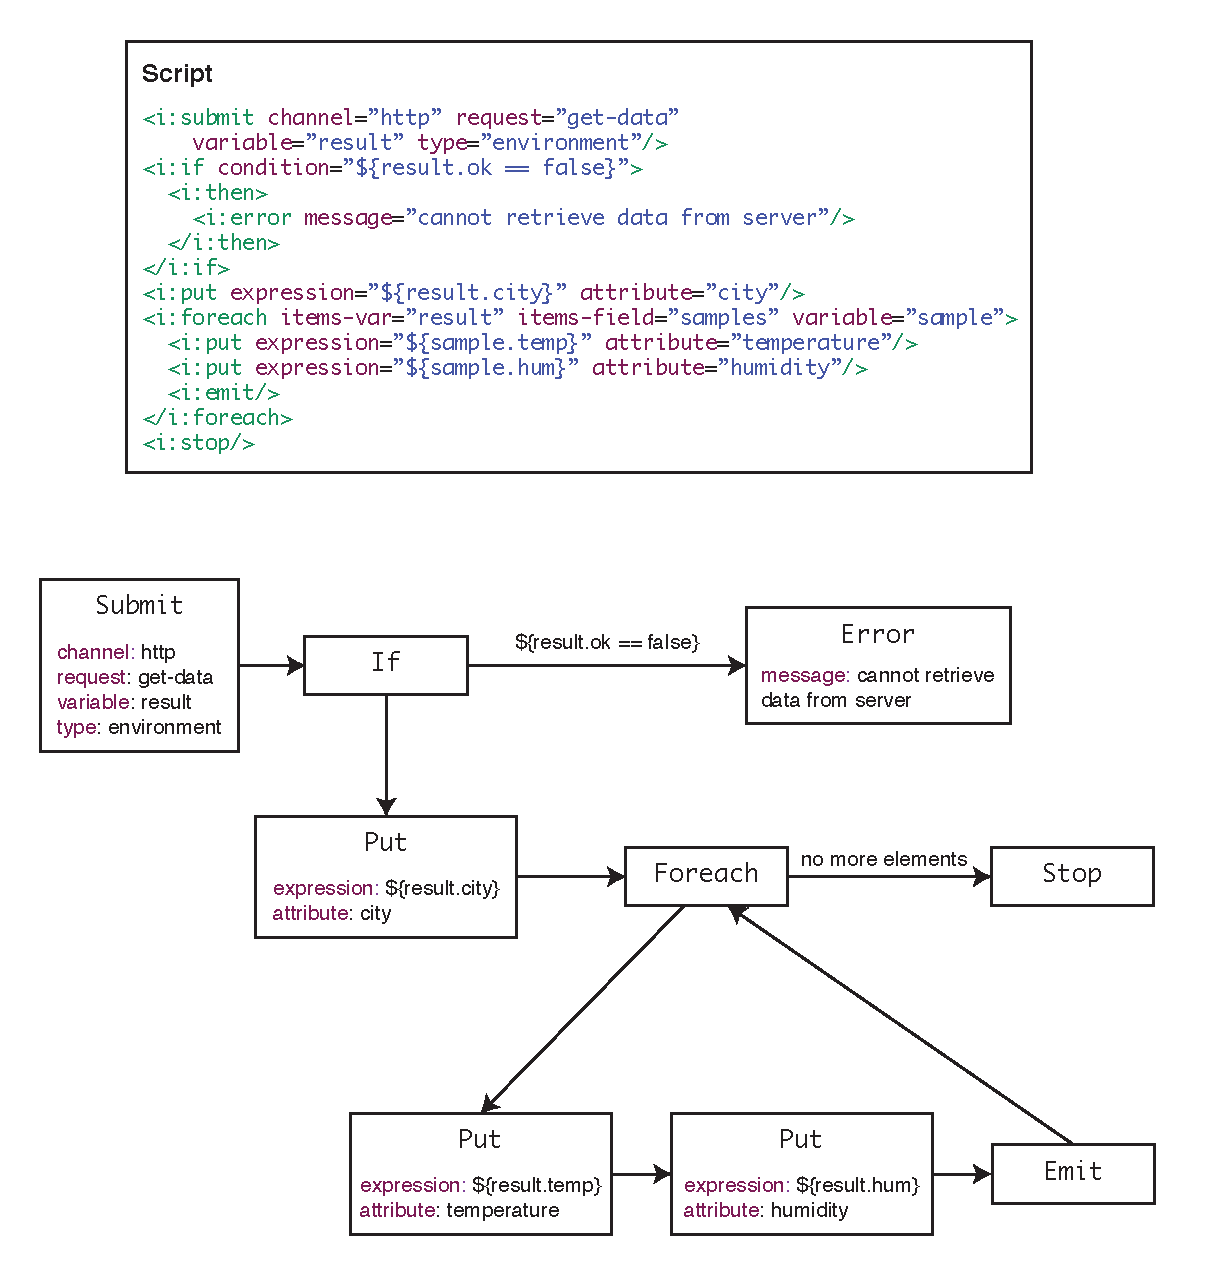
\includegraphics[width=\textwidth]{imgs/script_sir.pdf}
\caption{A PerLa \texttt{Script} and its corresponding SIR representation}
\end{figure}

Once started, PerLa \texttt{Scripts} are sandboxed in a dedicated thread of
execution. For better isolation, the current status of each running
\texttt{Script} instance is stored inside a private \texttt{ExecutionContext}
object, which contains the following elements:

\begin{itemize}

    \item \textbf{Program Counter:} A reference to the current instruction;

    \item \textbf{Variable Map:} An associative array that stores the current
        value of all declared variables;

    \item \textbf{Record staging area:} Temporary working area used to create
        new records;

    \item \textbf{Output records:} List of records to be returned when a
        \texttt{stop} instruction is encountered. 

\end{itemize}

This design ensures that all changes a single \texttt{Script} makes to its
environment will remain private, that its status won't be altered by any
other rogue routine, and that several \texttt{Scripts} can run simultaneously
without interfering with each other.

The execution of a \texttt{Script} is always subordinated to an external event,
like the submission of a new user request or the arrival of information from a
sensing device. In particular, PerLa \texttt{Scripts} associated with the
management of sensor data tend to run frequently and for a relatively short
period of time, as their execution is triggered by each sample collected from
the sensing network. To better cope with such usage scenario, the
\texttt{Script Engine} implements a thread caching mechanism that reduces
memory usage and startup times by reclaiming the runtime environment of each
terminated \texttt{Script}, and repurposing it for a new execution. This
caching technique greatly reduces the overall number of objects allocated by
the Java Virtual Machine, and guarantees that the overhead due to the
initialization of new \texttt{ExecutionContext} instances is shared between
multiple \texttt{Script} runs.

Moreover, the \texttt{Script Engine} can preemptively pause I/O bound
computations to optimize the usage of available system resources. This feature,
implemented by leveraging the asynchronous I/O design of the PerLa Middleware,
is totally transparent to the \texttt{Script} developer, who should not worry
with matters of concurrent programming; \texttt{Scripts} are automatically
paused after an \texttt{IORequest} is submitted to a \texttt{Channel}, and
their execution resumes as soon as the I/O activity terminates. These
two operations --- pause and resume --- are performed within the
\texttt{submit} instruction, which interrupts the \texttt{Script} after
an I/O request is submitted, and restarts it once the associated response is
available.


\section{Putting it all together: the FPC}

The \texttt{FPC} (Functionality Proxy Component) is the main data access
interface available to the PerLa Middleware. Its chief duty is to provide a
high-level abstraction of a Pervasive System by exposing the functionalities of
all devices of the network through a single consistent API. Every instance of
the PerLa Middleware hosts multiple \texttt{FPCs}, one for each sensing node.
This one-to-one relationship --- the fulcrum of the PerLa philosophy --- is a
fundamental architectural feature that endows the Middleware with utmost
flexibility and the finest granularity of control, as it presents final users
with the possibility to manage heterogeneous networks of sensing devices, down
to the single node, through a uniform set of high-level functions.

\begin{figure}[h!]
\center
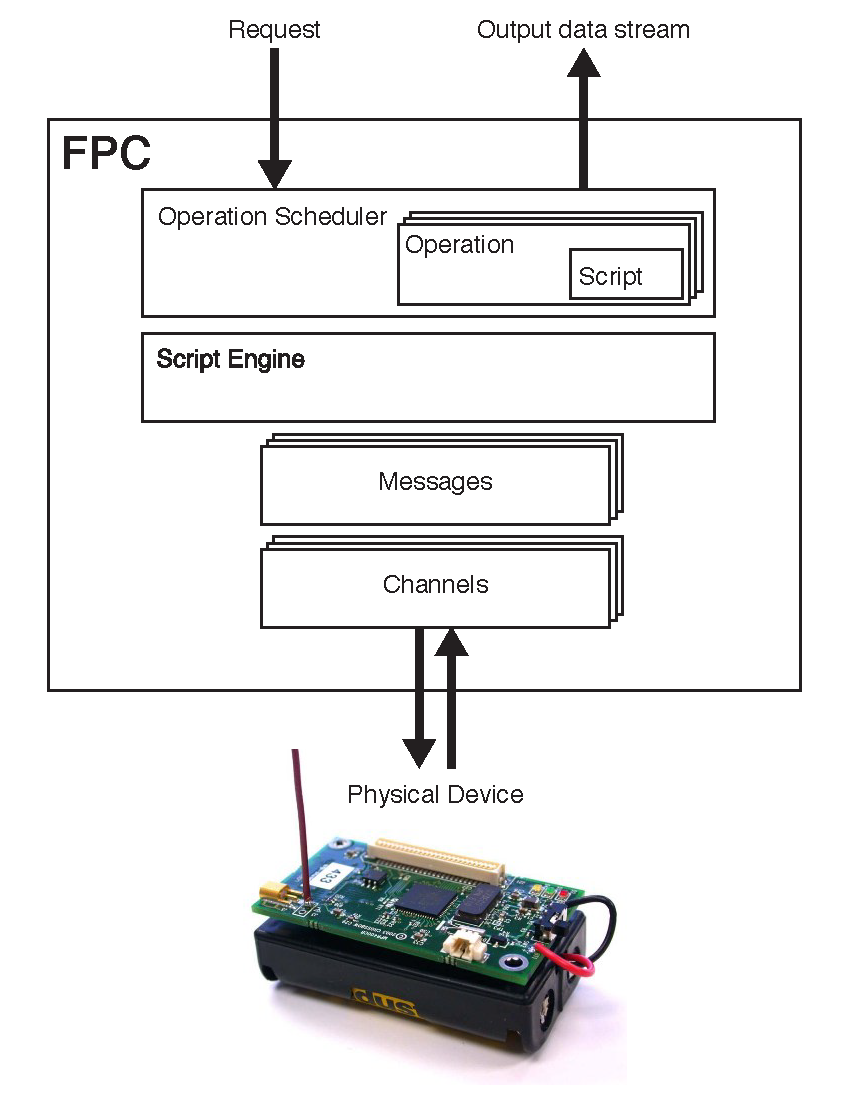
\includegraphics[width=0.6\textwidth]{imgs/fpc.pdf}
\caption{Internal structure of the Functionality Proxy Component}
\label{fig:fpc}
\end{figure}

\texttt{FPCs} are created from the composition of all Middleware components
described in the former sections of this chapter. As shown in
figure~\ref{fig:fpc}, these software modules are complemented by a set of
\texttt{Operations} and an \texttt{Operation Scheduler}. An \texttt{Operation}
is a collection of \texttt{Scripts} committed to the management of a well
defined aspect of an endpoint device, such as the retrieval of a specific data
sample at periodic intervals of time. In total, there are four different
\texttt{Operation} types available in the PerLa Middleware, each of which
corresponds to a \texttt{FPC} action (get, set, periodic sampling and
asynchronous event handling). Each of these \texttt{Operations} is associated
with the list of device \texttt{Attribute} that can be modified or generated
with it; this list is automatically inferred by the PerLa Middleware by
analyzing the associated data access \texttt{Scripts}.

\subsubsection{Get Operation}

A single \texttt{Script} that retrieves information from the remote device. It
can be used to perform a single-shot sampling operation or to read software
parameters stored on the connected endpoint.

This \texttt{Operation} type is introduced by the \lstinline!<get>! XML tag,
and contains a single PerLa \texttt{Script} that is responsible for connecting
with the remote device, retrieving the information requested by the user, and
creating an output record. The following example shows a textbook
implementation of the \texttt{Get Operation}, which demonstrates how all the
aforementioned operations can be performed in a few lines of PerLa
\texttt{Script}.

\lstset{language=XML}
\begin{lstlisting}
<get id="single-temp-sample">
  <i:submit request="temperature-request" channel="serial"
            variable="result" type="temperature-msg"/>
  <i:put expression="${result.temperature}" attribute="temperature"/>
  <i:emit/>
</get>
\end{lstlisting}

\subsubsection{Set Operation}

A single \texttt{Script} that sends information to the controlled device. It
can be used to dispatch commands, activate mechanisms, or change software
parameters on a remote sensing node.

All \texttt{Set Operation} \texttt{Scripts} must be enclosed in a
\lstinline!<set>! XML tag, and are required to define a series of actions
resulting in the transmission of data to the remote device. An example of this
\texttt{Operation} is available in the code excerpt below, which retrieves the
current time from a parameter passed by the \texttt{FPC} user
(\lstinline!arg['timestamp']!), and delivers it by means of a
\texttt{SerialChannel}.

\lstset{language=XML}
\begin{lstlisting}
<set id="set-clock">
  <i:create variable="settings" type="settings-msg"/>
  <i:set variable="settings" field="time" value="${arg['timestamp']}"/>
  <i:submit request="send-settings" channel="serial">
    <i:param name="payload" variable="settings"/>
  </i:submit>
</set>
\end{lstlisting}

\subsubsection{Periodic Operation}

A collection of \texttt{Scripts} for managing an unattended, periodic stream of
information. The \texttt{Periodic Operation} is more complicated than previous
\texttt{Operation} types, both from a syntactic and an operative point of view,
as it requires the device developer to specify three different classes of
\texttt{Scripts}.

The first of these is the \lstinline!<start>! \texttt{Script}, which is
employed to initialize the sampling operation. It normally contains a series of
instruction that parse the signal rate requested by the user, configure the
device to start the sampling operation, and handle potential error conditions.
By default, the sampling period exposed to the \texttt{Script} by means of the
\lstinline!arg['period']! argument is expressed in milliseconds; it is the
developer's duty to convert this value into whichever format is required by the
remote device. The code extract available below is worthy of note, since it is
employed to initialize two different sampling operations at once, one for
temperature, and one for humidity.

After the sampling operation is correctly initialized, the sensing node will
begin sending data packets towards its controlling \texttt{FPC}. All the
instructions required to convert these raw information into a record suitable
for further processing have to be specified inside an \lstinline!<on>! tag. As
shown below, each \texttt{Periodic Operation} is to be equipped with an
\lstinline!<on>! \texttt{Script} for each different type of \texttt{Message}
sent by the device.

Finally, the \texttt{Periodic Operation} is required to contain a
\lstinline!<stop>! \texttt{Script} that can be used to terminate the sampling
operation and undo any action performed at startup.

\lstset{language=XML}
\begin{lstlisting}
<periodic id="weather-periodic">
  <start>
    <i:create variable="period" type="sampling-period"/>
    <i:set variable="period" field="period" value="${arg['period']}"/>
    <i:submit request="temperature-request" channel="simulator">
            <i:param name="period" variable="period"/>
    </i:submit>
    <i:submit request="humidity-request" channel="simulator">
            <i:param name="period" variable="period"/>
    </i:submit>
  </start>
  <stop>
    <i:create variable="period" type="sampling-period"/>
    <i:set variable="period" field="period" value="0"/>
    <i:submit request="temperature-request" channel="simulator">
            <i:param name="period" variable="period"/>
    </i:submit>
    <i:submit request="humidity-request" channel="simulator">
            <i:param name="period" variable="period"/>
    </i:submit>
  </stop>
  <on message="temperature-msg" variable="result">
    <i:put expression="${result.temperature}" attribute="temperature" />
    <i:emit />
  </on>
  <on message="humidity-msg" variable="result">
    <i:put expression="${result.humidity}" attribute="humidity" />
    <i:emit />
  </on>
</periodic>
</periodic>
\end{lstlisting}

\subsubsection{Async Operation}

A collection of \texttt{Scripts} that handles an asynchronous stream of
information from the device, i.e. a series of events that are received at
irregular intervals of time. Similarly to the \texttt{Periodic Operation}, the
\texttt{Async Operation} features a \lstinline!<start>! \texttt{Script}
(optional), and a \lstinline!<on>! \texttt{Script} for each different type of
event message that may be received from the sensing node.

\lstset{language=XML}
\begin{lstlisting}
<async id="event-async">
  <start>
    <i:create variable="period" type="sampling-period"/>
    <i:set variable="period" field="period" value="200"/>
    <i:submit request="event-request" channel="simulator">
      <i:param name="period" variable="period"/>
    </i:submit>
  </start>
  <on message="event-msg" variable="result">
    <i:put expression="${result.event}" attribute="event"/>
    <i:emit />
  </on>
</async>
\end{lstlisting}


\subsection{The FPC interface}

The \texttt{FPC} interface, whose signature is available in
listing~\ref{lst:fpc}, represents one of the defining features of the PerLa
Middleware. Its technology-agnostic data access methods provide an easy and
intuitive way to access the information generated by a Pervasive System, and
require no knowledge of the underlying hardware layer in order to be used.

~\\
\lstset{language=java}
\begin{lstlisting}[caption=The FPC interface,label={lst:fpc}]
public interface Fpc {
    public int getId();

    public String getType();

    public Collection<Attribute> getAttributes();

    public Task set(Map<Attribute, Object> valueMap, TaskHandler handler);

    public Task get(Collection<Attribute> attributes, TaskHandler handler);

    public Task periodic(Collection<Attribute> attributes, long periodMs,
            TaskHandler handler);

    public Task async(Collection<Attribute> attributes, TaskHandler handler);
}
\end{lstlisting}

The first three methods of this interface --- \texttt{getId()},
\texttt{getType()} and \texttt{getAttributes()} --- are designed to retrieve a
series of basic information concerning the remote endpoint. The first one,
\texttt{getId()}, returns a numeric identifier that can be used to address the
single specific node connected to the current \texttt{FPC} object. The second
one, \texttt{getType()}, is employed to retrieve a brief textual description of
the remote endpoint. Lastly, the \texttt{getAttributes()} method returns a
comprehensive list of all device \texttt{Attributes} that can be sampled or
modified using an \texttt{FPC}, qualified in terms of name, data type
(\texttt{id}, \texttt{integer}, \texttt{float}, \texttt{string},
\texttt{boolean} or \texttt{timestamp}) and access permissions
(\texttt{read-only}, \texttt{read-write} or \texttt{write-only}).

\texttt{Attribute} values can be retrieved or set using the \texttt{FPC}'s data
access methods, namely \texttt{get()}, \texttt{periodic()}, \texttt{set()}, and
\texttt{async()}. Similarly to what already seen for other Middleware
components described in previous sections of this document, all these methods
implement the asynchronous interaction paradigm introduced in
section~\ref{sec:newmiddleware.async}. As shown in listing~\ref{lst:fpc}, their
immediate return type is in fact a \texttt{Task} object, which can be employed
to control the status of the ongoing data access operation. The actual data
samples and events generated by the \texttt{FPC} are notified asynchronously
through a \texttt{TaskHandler} using the following methods:

\begin{itemize}

    \item \textbf{complete():} Signals that the operation to which the
        \texttt{TaskHandler} is associated has just been completed. It is
        employed to notify the successful completion of a \texttt{set()}
        operation, or to indicate that a \texttt{get()} operation has been
        stopped and will not produce any new record;

    \item \textbf{newRecord():} Delivers a new record;

    \item \textbf{error():} Indicates that the operation associated to the
        \texttt{TaskHandler} was aborted due to an error.
\end{itemize}

~\\
\lstset{language=java}
\begin{lstlisting}[caption={The \texttt{Task} and \texttt{TaskHandler}
interfaces.},label={lst:task}]
public interface Task {
    public Collection<? extends Attribute> getAttributes();

    public boolean isRunning();

    public void stop();
}

public interface TaskHandler {
    public void complete(Task task);

    public void newRecord(Task task, Record record);

    public void error(Task task, Throwable cause);
}
\end{lstlisting}

When invoking one of the available data retrieval methods the user is always
required to list all \texttt{Attributes} to be sampled. This information is
employed by the \texttt{FPC} to check whether the requested information can be
gathered through the remote device or not, and to select an \texttt{Operation}
that best suits the user's demands. Both these activities are performed by the
\texttt{OperationScheduler}, a Middleware component tasked with managing all
the data handling \texttt{Operations} available in an \texttt{FPC}. This
component is also responsible for the management of concurrent sampling
operations occurring at different rates, a scenario that requires the
\texttt{OperationScheduler} to start a single periodic \texttt{Operation} using
the highest requested sampling frequency, and to distribute the resulting
records according to the requirements of each single user. An additional thing
of note on the \texttt{OperationScheduler} is its ability simulate a periodic
sampling activity by executing a single-shot \texttt{Get Operation} repeatedly.


\subsection{FPC Factory}

As suggested by the name, the 

\subsection{Registry}


\subsection{Complete XML Device Descriptor examples}

\textbf{Example 1}

The Device Descriptor portrayed in this first example is employed to create a
Simulator \texttt{FPC}, a useful tool that helps testing the PerLa Middleware
even when no physical sensor nodes are available. This simulated device exposes
two attributes: a read-only float representing the temperature in Celsius
degrees (\texttt{temp\_c}), and a write-only integer that will be used to set
the sampling period (\texttt{period}).

This \texttt{FPC} contains one \texttt{Channel} of type
\texttt{SimulatorChannel}, which generates new data samples without requiring a
connection to a real sensing device. In our example, the
\texttt{SimulatorChannel} is configured with a single data generation routine,
named \texttt{temperature}, that automatically creates new data samples in
increments of 0.1\degree, spanning from a minimum of 16\degree~C to a maximum
of 20\degree~C. The \lstinline!<request>! section shows that a single
\texttt{IORequest} object is enough to drive the single data generator
available in this \texttt{FPC}.

Only two \texttt{Message} types are declared in the Device Descriptor: a
\texttt{temperature-msg} message, which contains a single field of type
\texttt{float}, and a \texttt{sampling-period} message, composed of only an
\texttt{integer} field. These two messages will be used to collect temperature
samples and to set the desired sampling period in the \texttt{SimulatorChannel}
respectively.

As can be seen from the \lstinline!<operation>! section of this descriptor, the
simulator device exposes a periodic sampling operation named
\texttt{temp-periodic}. It is important to note that the \texttt{start Script}
initializes the \texttt{SimulatorChannel} according to the sampling rate
specified by the user, which is retrieved with a \lstinline!${arg['period']}!
expression. New output records are create by the \texttt{on Script} upon
arrival of each \texttt{temperature-msg}. Finally, the generation of new data
samples can be stopped by setting the sampling frequency to zero.

~\\
\lstset{language=XML}
\begin{lstlisting}
<?xml version="1.0" encoding="UTF-8"?>
<device type="Weather simulator"
    xmlns="http://perla.dei.org/device"
    xmlns:i="http://perla.dei.org/device/instructions"
    xmlns:sim="http://perla.dei.org/channel/simulator">

  <attributes>
    <attribute id="temp_c" type="float" permission="read-only"/>
    <attribute id="period" type="integer" permission="write-only"/>
  </attributes>

  <channels>
    <sim:channel id="simulator">
      <sim:generator id="temperature">
        <sim:field name="temperature" strategy="step"
                   type="float" min="16" max="20" increment="0.1"/>
        </sim:generator>
    </sim:channel>
  </channels>
  
  <messages>
    <sim:message id="temperature-msg">
      <sim:field name="temperature" type="float"/>
    </sim:message>
    <sim:message id="sampling-period">
      <sim:field name="period" type="integer"/>
    </sim:message>
  </messages>
  
  <requests>
    <sim:request id="temperature-request" generator="temperature"/>
  </requests>
  
  <operations>
    <periodic id="temp-periodic">
      <start>
        <i:create variable="period" type="sampling-period"/>
        <i:set variable="period" field="period" value="${arg['period']}"/>
        <i:submit request="temperature-request" channel="simulator">
          <i:param name="period" variable="period"/>
        </i:submit>
      </start>
      <stop>
        <i:create variable="period" type="sampling-period"/>
        <i:set variable="period" field="period" value="0"/>
        <i:submit request="temperature-request" channel="simulator">
          <i:param name="period" variable="period"/>
        </i:submit>
      </stop>
      <on message="temperature-msg" variable="result">
        <i:put expression="\${result.temperature}" attribute="temp_c" />
        <i:emit />
      </on>
    </periodic>
  </operations>

</device>
\end{lstlisting}

\textbf{Example 2}

This second Device Descriptor is used to configure an \texttt{FPC} for
collecting data from a RESTful meteorological service. The remote API is
accessed by means of a \texttt{HTTPChannel}, which retrieves a complete
JSON-encoded weather report for the city of Milan.

The service chosen for this application returns its results using a fairly
complex JSON entity, whose structure has been replicated in the
\lstinline!<message>! section of this descriptor. The main \texttt{weather}
object is in fact a wrapper for three other components: a \texttt{coord}
message, a \texttt{data} message, and a \texttt{wind} message. It is worth
noting that these three sub-objects are constructed using only primitive
fields, and that they are not intended to be used on their own; their only
purpose is to be included as the constituent elements of a \texttt{weather}
message.

The stateless nature of the HTTP protocol is underscored by the simplicity of
the \texttt{HTTPChannel} declaration, which doesn't require any parameter
except for its own identifier, and by the related \texttt{HTTPIORequest}, where
all information required for querying the RESTful API endpoint is stored. These
two \texttt{FPC} components are then employed in the \lstinline!<get>!
\texttt{Operation}, which is tasked with creating a new record from the
\texttt{weather} object retrieved from the web service. 

~\\
\lstset{language=XML}
\begin{lstlisting}
<?xml version="1.0" encoding="UTF-8"?>
<device type="REST Weather station"
    xmlns="http://perla.dei.org/device"
    xmlns:js="http://perla.dei.org/fpc/message/json"
    xmlns:http="http://perla.dei.org/channel/http"
    xmlns:i="http://perla.dei.org/device/instructions">

  <attributes>
    <attribute id="city" type="string" permission="read-only"/>
    <attribute id="temp_k" type="float" permission="read-only"/>
    <attribute id="temp_c" type="float" permission="read-only"/>
    <attribute id="temp_f" type="float" permission="read-only"/>
    <attribute id="pressure" type="float" permission="read-only"/>
    <attribute id="humidity" type="float" permission="read-only"/>
    <attribute id="wind_speed" type="float" permission="read-only"/>
    <attribute id="wind_deg" type="float" permission="read-only"/>
  </attributes>

  <channels>
    <http:channel id="http"/>
  </channels>

  <messages>
    <js:object id="coord">
      <js:value name="lon" type="string"/>
      <js:value name="lat" type="string"/>
    </js:object>

    <js:object id="data">
      <js:value name="temp" type="float"/>
      <js:value name="pressure" type="float"/>
      <js:value name="humidity" type="float"/>
      <js:value name="temp_min" type="float"/>
      <js:value name="temp_max" type="float"/>
    </js:object>

    <js:object id="wind">
      <js:value name="speed" type="float"/>
      <js:value name="deg" type="float"/>
    </js:object>

    <js:object id="weather">
      <js:value name="coord" type="coord"/>
      <js:value name="data" type="data"/>
      <js:value name="wind" type="wind"/>
    </js:object>
  </messages>

  <requests>
    <http:request id="weather-mi"
                  host="http://api.openweathermap.org/data/2.5/weather?q=Milan,it"
                  method="get" />
  </requests>

  <operations>
    <get id="weather-mi">
      <i:submit request="weather-mi" channel="http"
                variable="result" type="weather"/>
      <i:put expression="Milan" attribute="city"/>
      <i:put expression="${result.data.temp}" attribute="temp_k"/>
      <i:put expression="${result.data.temp - 272.15}" attribute="temp_c"/>
      <i:put expression="${(result.data.temp - 273.15) * 9 / 5 + 32}"
             attribute="temp_f"/>
      <i:put expression="${result.data.pressure}" attribute="pressure"/>
      <i:put expression="${result.data.humidity}" attribute="humidity"/>
      <i:put expression="${result.wind.speed}" attribute="wind_speed"/>
      <i:put expression="${result.wind.deg}" attribute="wind_deg"/>
      <i:emit/>
    </get>
  </operations>

</device>
\end{lstlisting}

\textbf{Example 3}

A purely educational Device Descriptor designed to showcase the following PerLa
Middleware features:

\begin{itemize}
    \item read-write, read-only write-only and static attributes;
    \item \texttt{SimulatorChannel} value generator configurations for all
        available data types;
    \item \texttt{Get} and \texttt{Set Operations};
    \item \texttt{Periodic Operations} with single and multiple
        \lstinline!<on>! \texttt{Scripts}.
\end{itemize}

~\\
\lstset{language=XML}
\begin{lstlisting}
<?xml version="1.0" encoding="UTF-8"?>
<device type="test"
    xmlns="http://perla.dei.org/device"
    xmlns:i="http://perla.dei.org/device/instructions"
    xmlns:sim="http://perla.dei.org/channel/simulator">

  <attributes>
    <attribute id="integer" type="integer" permission="read-write"/>
    <attribute id="float" type="float" permission="read-write"/>
    <attribute id="boolean" type="boolean" permission="read-write"/>
    <attribute id="string" type="string" permission="read-write"/>
    <attribute id="event" type="boolean" permission="read-only"/>
    <attribute id="period" type="integer" permission="write-only"/>
    <attribute id="static" type="integer" access="static" value="5"/>
  </attributes>

  <channels>
    <sim:channel id="simulator">
      <sim:generator id="all">
        <sim:field name="type" strategy="static" value="all"/>
        <sim:field name="integer" strategy="dynamic"
                   type="integer" min="12" max="32"/>
        <sim:field name="float" strategy="dynamic"
                   type="float" min="450" max="600"/>
        <sim:field name="string" strategy="dynamic"
                   type="string" min="10" max="15"/>
      </sim:generator>
      <sim:generator id="integer">
        <sim:field name="type" strategy="static" value="integer"/>
        <sim:field name="integer" strategy="dynamic"
                   type="integer" min="47" max="58"/>
      </sim:generator>
      <sim:generator id="string">
          <sim:field name="type" strategy="static" value="integer"/>
          <sim:field name="string" strategy="dynamic"
                     type="string" min="5" max="5"/>
      </sim:generator>
      <sim:generator id="boolean">
        <sim:field name="type" strategy="static" value="boolean"/>
        <sim:field name="boolean" strategy="dynamic" type="boolean"/>
      </sim:generator>
      <sim:generator id="event">
        <sim:field name="type" strategy="static" value="event"/>
        <sim:field name="event" strategy="dynamic" type="boolean"/>
      </sim:generator>
    </sim:channel>
  </channels>

  <messages>
    <sim:message id="set-msg">
      <sim:field name="test" type="integer"/>
    </sim:message>
    <sim:message id="sampling-period">
      <sim:field name="period" type="integer"/>
    </sim:message>
    <sim:message id="all-msg">
      <sim:field name="type" type="string" qualifier="static" value="all"/>
      <sim:field name="integer" type="integer"/>
      <sim:field name="float" type="float"/>
      <sim:field name="string" type="string"/>
    </sim:message>
    <sim:message id="integer-msg">
      <sim:field name="type" type="string" qualifier="static" value="integer"/>
      <sim:field name="integer" type="integer"/>
    </sim:message>
    <sim:message id="string-msg">
      <sim:field name="type" type="string" qualifier="static" value="string"/>
      <sim:field name="string" type="string"/>
    </sim:message>
    <sim:message id="boolean-msg">
      <sim:field name="type" type="string" qualifier="static" value="boolean"/>
      <sim:field name="boolean" type="boolean"/>
    </sim:message>
    <sim:message id="event-msg">
      <sim:field name="type" type="string" qualifier="static" value="event"/>
      <sim:field name="event" type="boolean"/>
    </sim:message>
  </messages>

  <requests>
    <sim:request id="all-request" generator="all"/>
    <sim:request id="integer-request" generator="integer"/>
    <sim:request id="string-request" generator="string"/>
    <sim:request id="boolean-request" generator="boolean"/>
    <sim:request id="event-request" generator="event"/>
  </requests>

  <operations>
    <get id="integer-get">
      <i:submit request="integer-request"
                channel="simulator" variable="result" type="integer-msg"/>
      <i:put expression="${result.integer}" attribute="integer"/>
      <i:emit/>
    </get>
    <get id="string-get">
      <i:submit request="string-request"
                channel="simulator" variable="result" type="string-msg"/>
      <i:put expression="${result.string}" attribute="string"/>
      <i:emit/>
    </get>
    <set id="integer-set">
      <!-- Just for test purposes -->
      <i:create variable="set-data" type="set-msg"/>
      <i:set variable="set-data" field="test" value="${param['integer']}"/>
    </set>
    <periodic id="all-periodic">
      <start>
        <i:create variable="period" type="sampling-period"/>
        <i:set variable="period" field="period" value="${param['period']}"/>
        <i:submit request="all-request" channel="simulator">
          <i:param name="period" variable="period"/>
        </i:submit>
      </start>
      <stop>
        <i:create variable="period" type="sampling-period"/>
        <i:set variable="period" field="period" value="0"/>
        <i:submit request="all-request" channel="simulator">
          <i:param name="period" variable="period"/>
        </i:submit>
      </stop>
      <on message="all-msg" variable="result">
        <i:put expression="${result.integer}" attribute="integer" />
        <i:put expression="${result.float}" attribute="float" />
        <i:put expression="${result.string}" attribute="string" />
        <i:emit />
      </on>
    </periodic>
    <periodic id="multiple-periodic">
      <start>
        <i:create variable="period" type="sampling-period"/>
        <i:set variable="period" field="period" value="${param['period']}"/>
        <i:submit request="integer-request" channel="simulator">
          <i:param name="period" variable="period"/>
        </i:submit>
        <i:submit request="boolean-request" channel="simulator">
          <i:param name="period" variable="period"/>
        </i:submit>
      </start>
      <stop>
        <i:create variable="period" type="sampling-period"/>
        <i:set variable="period" field="period" value="0"/>
        <i:submit request="integer-request" channel="simulator">
          <i:param name="period" variable="period"/>
        </i:submit>
        <i:submit request="boolean-request" channel="simulator">
          <i:param name="period" variable="period"/>
        </i:submit>
      </stop>
      <on message="integer-msg" variable="result" sync="true">
        <i:put expression="${result.integer}" attribute="integer" />
        <i:emit />
      </on>
      <on message="boolean-msg" variable="result">
        <i:put expression="${result.boolean}" attribute="boolean" />
        <i:emit />
      </on>
    </periodic>
    <async id="event-async">
      <start>
        <i:create variable="period" type="sampling-period"/>
        <i:set variable="period" field="period" value="200"/>
        <i:submit request="event-request" channel="simulator">
          <i:param name="period" variable="period"/>
        </i:submit>
      </start>
      <on message="event-msg" variable="result">
        <i:put expression="${result.event}" attribute="event"/>
        <i:emit />
      </on>
    </async>
  </operations>

</device>
\end{lstlisting}

